\chapter{Biohadoop Architecture}
\label{chap:impl}

Biohadoop is a framework to parallelize algorithms on Apache Hadoop. It works according to the master-worker principle where one master commands several workers. The master runs an algorithm whose compute intensive parts are executed by the workers in parallel.

% The genetic algorithm (GA) from chapter \ref{chap:bioalgorithms:ga} is used in the following sections as an example of how to parallelize an algorithm for the master-worker scheme. 
In the following, we are going to show how to parallelize the GA from chapter \ref{chap:bioalgorithms:ga}. A GA is an iterative procedure, each iteration creates a set of new individuals, called offsprings, evaluates their fitness and selects the best individuals for the next iteration based on the fitness of all GA individuals. The creation of an offspring and its subsequent fitness evaluation can be combined into a single function. This function consumes most of the time in a GA and can be executed in parallel since it depends only on its input values (the parents) and has no side effects. Therefore it is a good example for a parallel task that can be performed by workers. The master controls the generational loop and workers create and evaluate individuals (see figure \ref{fig:master-worker}).

% , while the rest of the GA algorithm runs on the master (see figure \ref{fig:master-worker}).

\begin{figure}
  \centering
  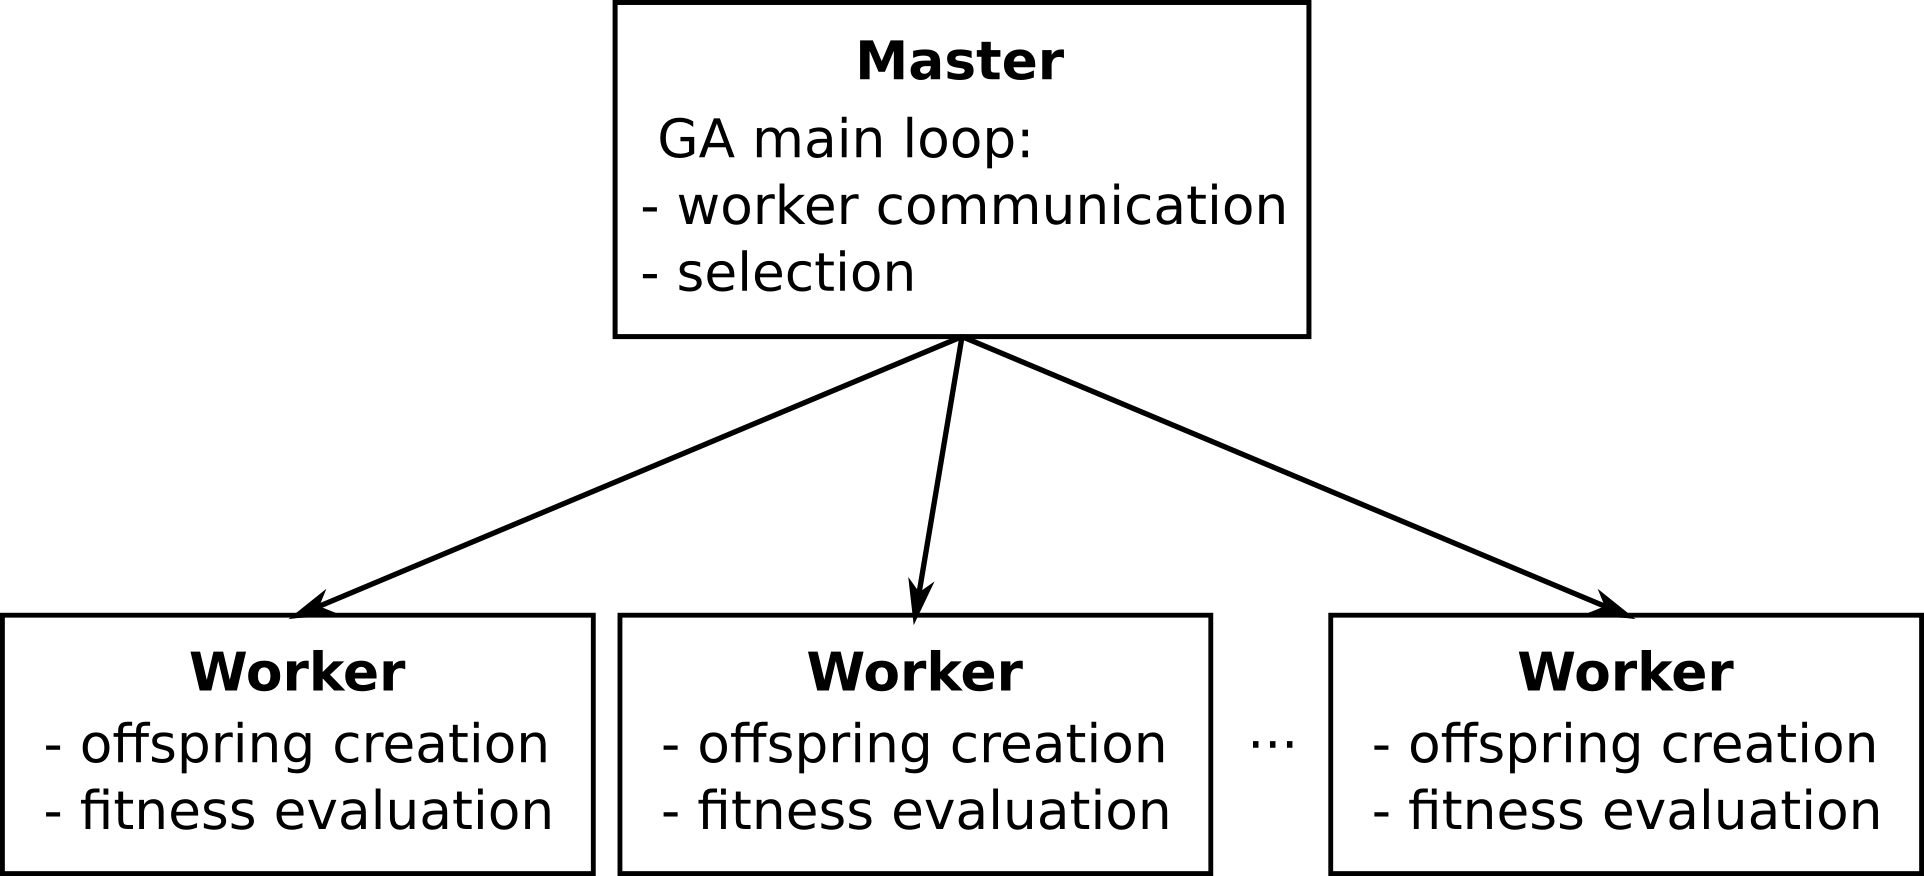
\includegraphics[width=100mm,natwidth=1924,natheight=876]{master-worker.png}
  \caption[Master-worker principle applied to GA]{Master-worker principle applied to a GA. One master commands several workers. The master runs the main loop, where it communicates with the workers to get new individuals. Then, it selects the best individuals to create the population of the next iteration.}
  \label{fig:master-worker}
\end{figure}

The master-worker architecture was chosen for Biohadoop, because many bio-inspired algorithms can be parallelized by this approach (like GA and PSO of chapter \ref{chap:bioalgorithms}). Another reason is that the master-worker scheme maps very well to YARN (see chapter \ref{chap:hadoop:yarn}).

Biohadoop is written to run as a YARN application and supports features that are not provided by YARN, such as:

\begin{itemize}
  \item Support for the execution of several algorithms at the same time in a single Biohadoop instance. This has the advantage that workers, and therefore resources, can be shared by the algorithms. It guarantees also that the algorithms run at the same time. This guarantee can't be given when several Biohadoop instances are used, as YARN decides when it executes a scheduled application. The island model (section \ref{chap:bioalgorithms:island-model}) benefits from this feature, as it ensures the simultaneous execution of the islands.
  \item Asynchronous communication between master and workers using Biohadoops task system (section \ref{chap:impl:task-system}). YARN doesn't provide a default communication facility between its containers.
  \item Storage and load of arbitrary data sets to and from a file system (section \ref{chap:impl:persistence}).
  \item Support for the island model, a high level parallelization that can be used to improve the optimization performance of bio-inspired optimization techniques by exchanging results between multiple instances of an algorithm (section \ref{chap:impl:island-model}).
  \item Support for Apache Oozie through a custom action (section \ref{chap:impl:oozie}). This custom action can be used to schedule one or many Biohadoop instances. It also allows the usage of Biohadoop in a larger workflow.
\end{itemize}

Every YARN application needs a client that submits the application to YARN. The YARN client in Biohadoop is implemented in the class \texttt{BiohadoopClient}. It is the main entrance point to run Biohadoop in a Hadoop environment and responsible to start the ApplicationMaster under the control of Hadoop.

Biohadoops ApplicationMaster starts the configured workers using additional YARN containers, and, since it is the master in the master-worker scheme, it executes the configured algorithms in this single ApplicationMaster instance and communicates with the workers. The ApplicationMasters main class is \texttt{BiohadoopApplicationMaster}. In a local (development) environment, it acts as the main entrance point to run Biohadoop without Hadoop (more on how to run Biohadoop can be found in appendix \ref{chap:usage:run}).

The workers are started in additional YARN containers. Each worker resides in a dedicated container.

Figure \ref{fig:architecture} shows how Biohadoops architecture maps to the architecture of a typical YARN application. It also gives a first impression of the task system that hides the technical details of the master-worker scheme from the algorithm. The task system consists of a task broker, one ore more endpoints and one or more workers.

\begin{figure}
  \centering
  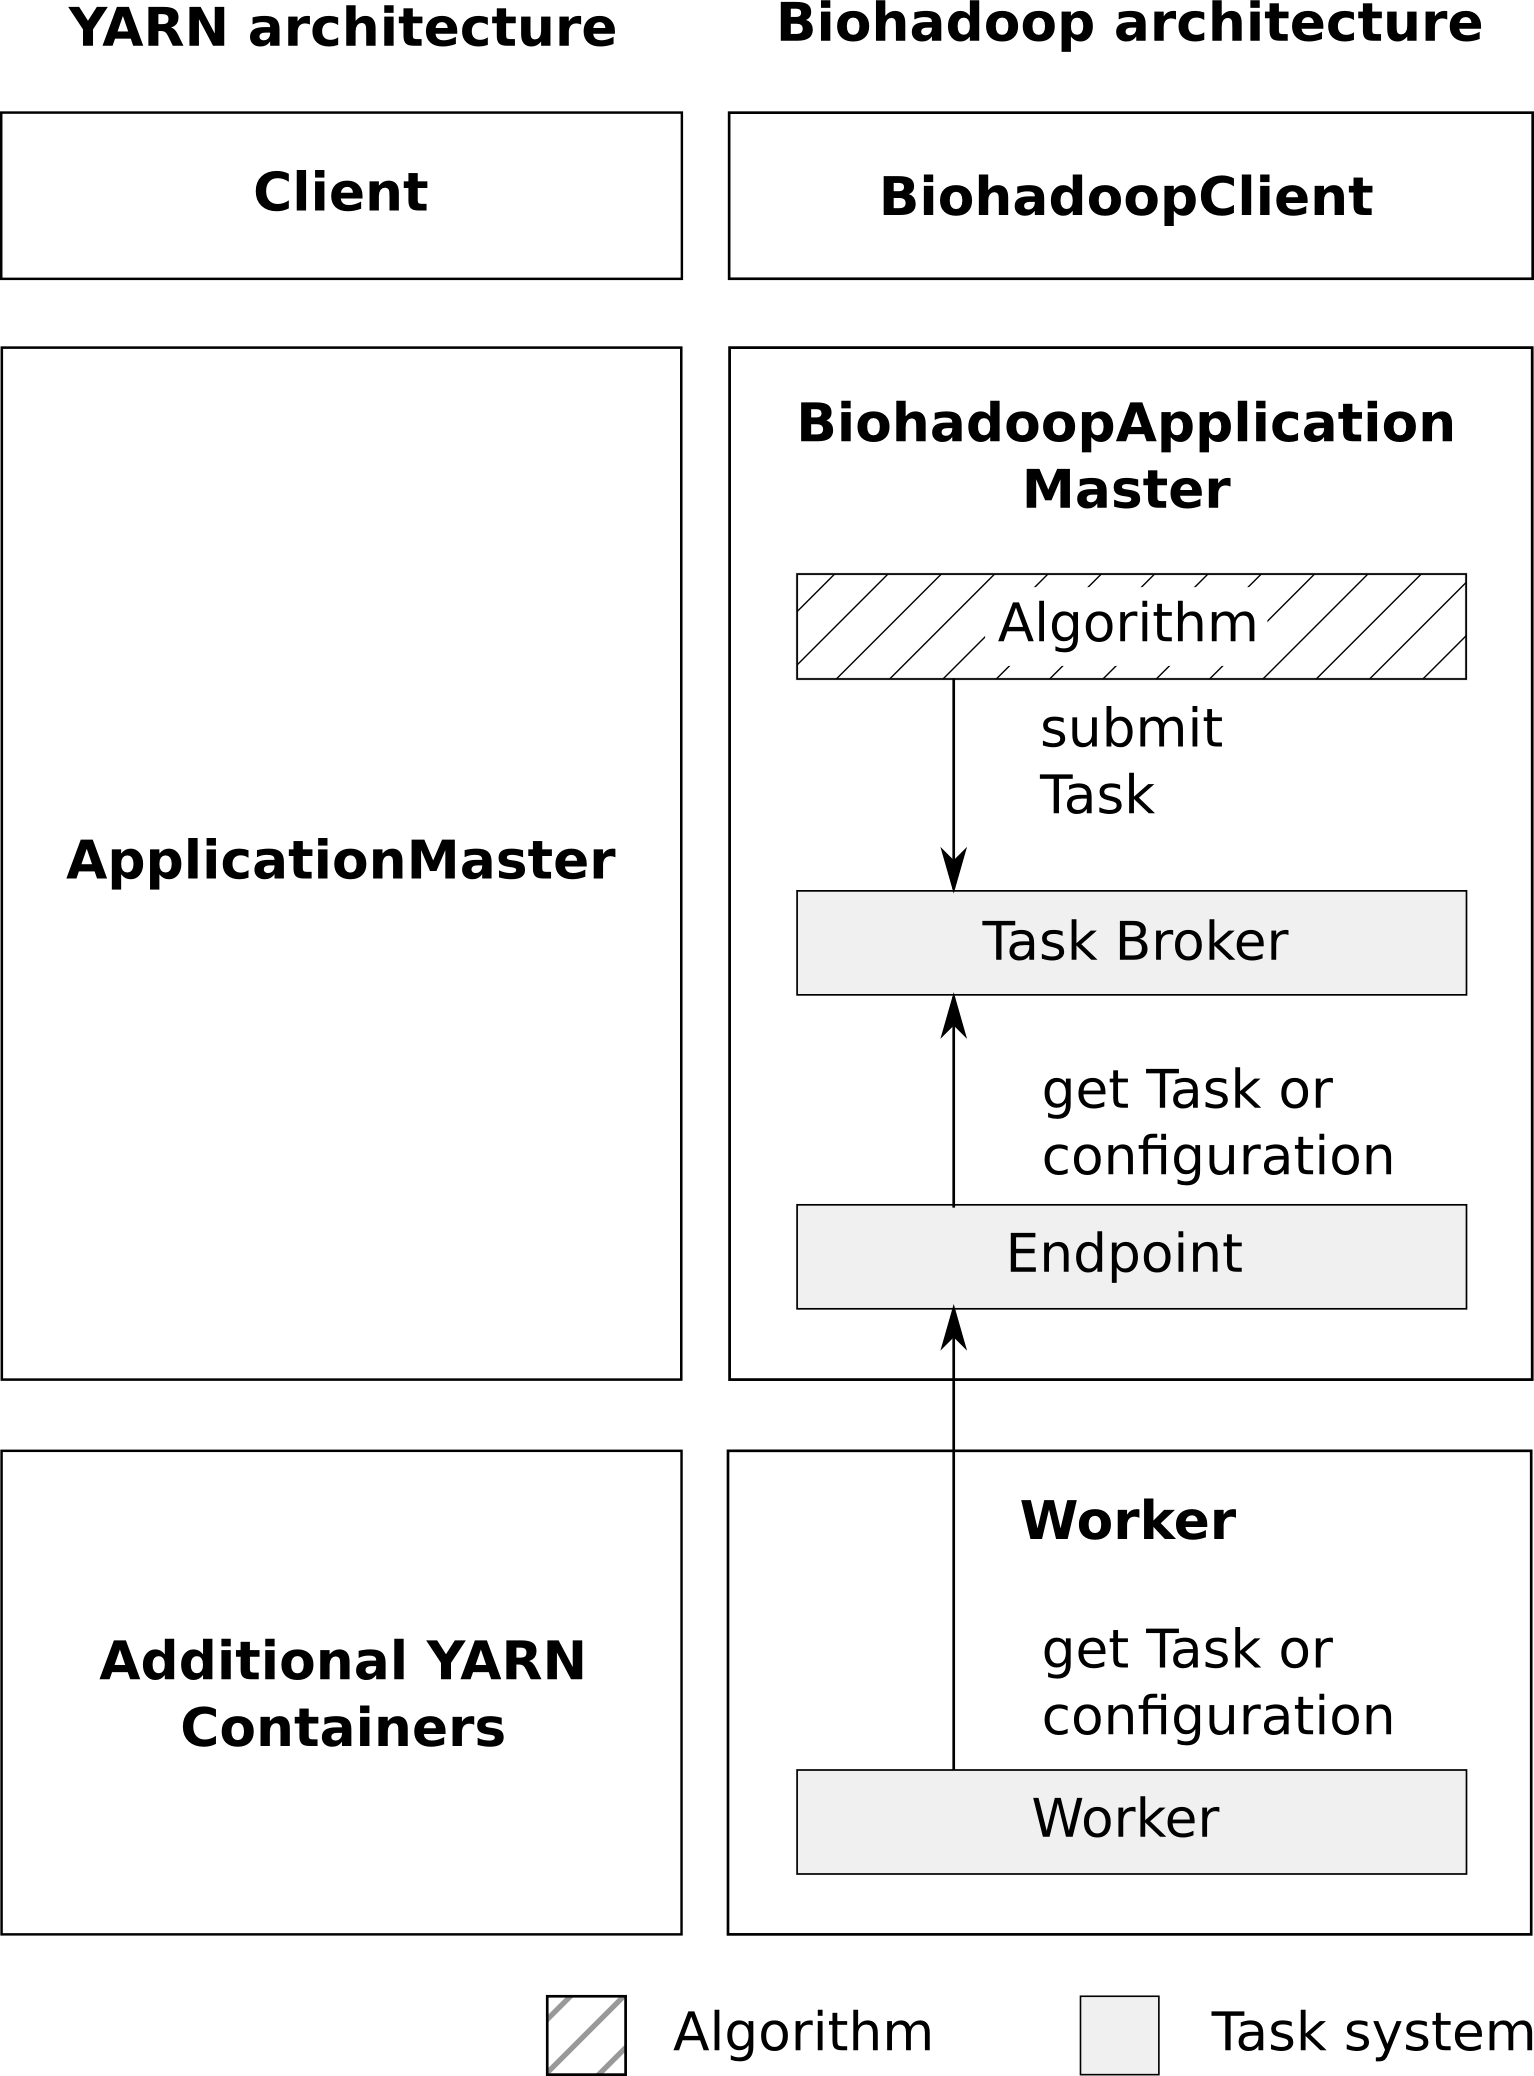
\includegraphics[width=80mm,natwidth=1534,natheight=2076]{architecture.png}
  \caption[Mapping of Biohadoops architecture to the architecture of a typical YARN application]{Mapping of Biohadoops architecture to the architecture of a typical YARN application}
  \label{fig:architecture}
\end{figure}

An algorithm uses the task system to submit work items, from here on called tasks, to the workers and to wait for the results. A task contains data and a reference to a task configuration. A task configuration defines how to compute the result for the task. In the GA example, a task would be to create individuals and compute their fitness. In this case, the task data represents the parent individuals that are used to create an offspring. The configuration defines the method for offspring creation and fitness computation.

Submitted tasks are queued by the task broker. Endpoints get tasks from the broker and send them to waiting workers. The workers execute the configured computations on the tasks and return the results to the endpoints, that promote the results back to the broker and from there to the algorithms.

A task configuration is usually shared by many tasks, for example each task in the GA uses the same method to compute an offspring and its fitness value. Therefore, a task configuration is send to a worker only the first time it is needed, and cached by the worker otherwise. This reduces the communication amount between the master and the workers.

Figure \ref{fig:task-conf-reuse} shows how a worker requests tasks or task configurations to compute the result for a task. The worker requests a task from the master (fig. \ref{fig:task-conf-reuse}(a)) which is delivered (fig. \ref{fig:task-conf-reuse}(b)). The worker then recognizes that it doesn't know how to compute the result for the task. Therefore, it has to request the task configuration (fig. \ref{fig:task-conf-reuse}(c)). The task configuration is returned (fig. \ref{fig:task-conf-reuse}(d)). The worker can now compute the task result (fig. \ref{fig:task-conf-reuse}(e)). The result is returned (fig. \ref{fig:task-conf-reuse}(f)) together with the request for the next task. The next task is delivered (fig. \ref{fig:task-conf-reuse}(g)) and as it uses the same task configuration as the prior task, the worker can reuse this configuration and directly compute the result (fig. \ref{fig:task-conf-reuse}(h)), after which the result is returned together with the request for the next task. More details about the task system can be found in section \ref{chap:impl:task-system}.

\begin{figure}
  \centering
  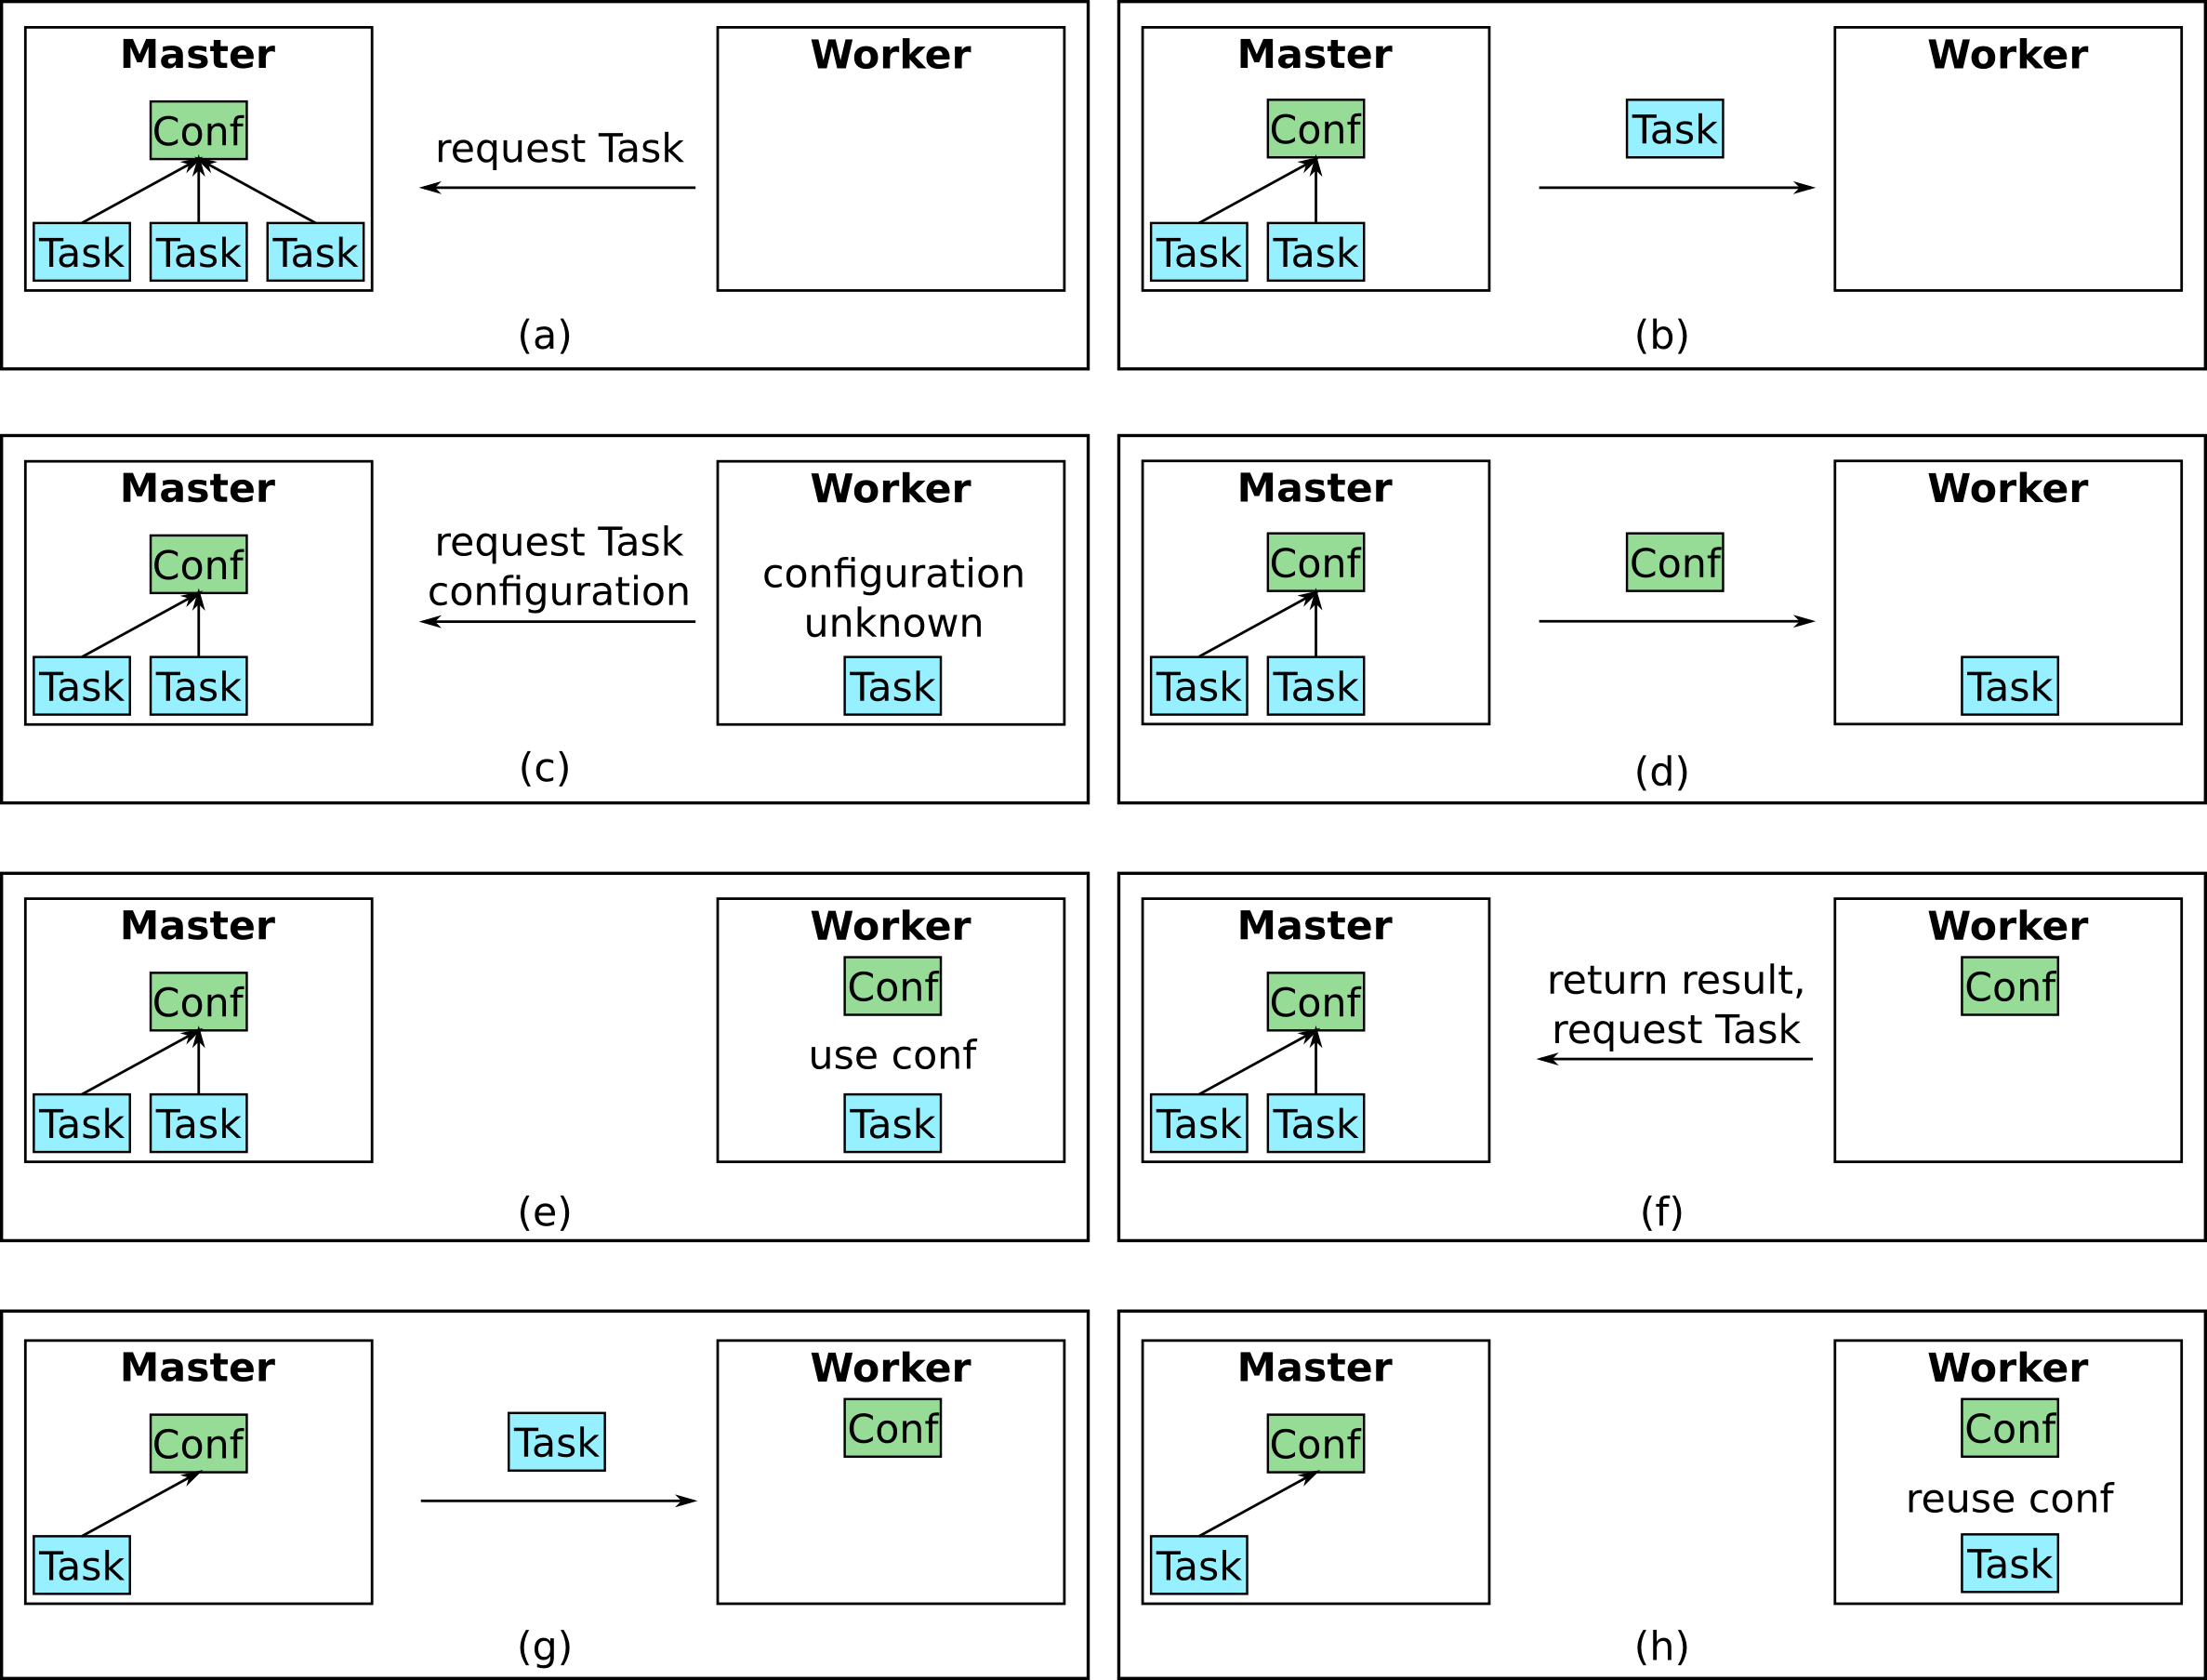
\includegraphics[width=130mm,natwidth=2374,natheight=1807]{task-conf-reuse.png}
  \caption[Task requests performed by a worker]{Task requests performed by a worker. The task configuration is send to the worker on demand.}
  \label{fig:task-conf-reuse}
\end{figure}

Persistence is another feature provided by Biohadoop. It can be used to save and load arbitrary data sets to and from the file system. This is convenient in many cases, e.g., if an algorithm wants to save its current state and reload this state at the next startup. To get more information about the persistence refer to section \ref{chap:impl:persistence}.

Biohadoop is capable of running several algorithms at the same time in a single Biohadoop instance. They all run in the same JVM as Biohadoop does, and can be of arbitrary type. For example it is possible to run two GA instances and one PSO instance at the same time. Since YARN doesn't guarantee when an application runs, the mentioned capability of launching several algorithms at the same time in the same JVM is a useful enhancement when it comes to high level parallelization using the island model. It guarantees that the algorithms really run at the same time. If the algorithms are started as separate Biohadoop instances, it is possible that they run in sequential order, instead of running at the same time.

But Biohadoop doesn't restrict the usage of the island model to algorithms that run in the same JVM. Algorithms that register to ZooKeeper \footnote{\url{http://zookeeper.apache.org/} last access: 05.09.2014} find each other also across the boundaries of different Biohadoop instances. The registration and data exchange is hidden behind Biohadoops island model API (see section \ref{chap:impl:island-model}). The execution of algorithms in different Biohadoop instances can lead to higher scalability, since each instance gets its own resources. However, it entails the aforementioned problem that YARN doesn't guarantee the order of execution, so a compromise has to be made.

Biooozie (section \ref{chap:impl:oozie}) implements a custom action for Apache Oozie and is used to run Biohadoop as part of a larger workflow. As an example, a workflow imports data from a set of sensors into HDFS, performs a MapReduce task on this data to extract the relevant information and executes Biohadoop to find a solution for a given problem.
% The action schedules a single Biohadoop instance or several instances in parallel, depending on its configuration.

In the following sections of this chapter Biohadoop is described in more detail, starting with the notion of Algorithm in section \ref{chap:impl:algorithm}. Section \ref{chap:impl:task-system} presents the task system and its components, followed by the description of the communication mechanisms in section \ref{chap:impl:communication}. The extensions section \ref{chap:impl:extensions} provides information about Biohadoops support for persistence and the island model. Section \ref{chap:impl:configuration} explains how to configure Biohadoop. Finally, Biooozie is presented in the section \ref{chap:impl:oozie}.
% Information on how to use Biohadoop can be found in chapter \ref{chap:usage}.

\section{Algorithm}
\label{chap:impl:algorithm}
An algorithm in terms of Biohadoop is the implementation of an abstract problem that should be solved. For example, a genetic algorithm (GA) can be implemented to solve an optimization problem.

Biohadoop provides an easy way to parallelize the algorithm using its asynchronous task system (see section \ref{chap:impl:task-system}). The algorithm can submit tasks to the task system that takes care about the distribution and computation of the tasks, and promotes the results back to the algorithm. The technical details of the task system are hidden from the algorithm.

Additional mechanisms that are offered to algorithms include persistence and high level parallelization using an island model (see section \ref{chap:impl:extensions}).

All those capabilities can be used by the algorithm, which must implement the \texttt{Algorithm} interface. This interface defines one method, namely \texttt{run}, which is invoked by Biohadoop after the system initialization has completed. The return value of the \texttt{run} method is void as there is no return data that could be used in a general way.

It is possible to run several algorithms of any kind simultaneously in one Biohadoop instance (e.g. two GA and one PSO). This is just a matter of configuration (see section \ref{chap:impl:configuration}).
   
If an error occurred during the execution of an algorithm, the algorithm may throw a \texttt{AlgorithmException}. The meaning of a thrown \texttt{AlgorithmException} is, that there was an unrecoverable error which prevented the algorithm to continue, but the programmer was aware that such an error could happen, e.g., when a needed configuration argument is missing. Sometimes an algorithm may throw an unchecked exception, like the \texttt{NullPointerException}. The difference to the \texttt{AlgorithmException} lies in the semantics: unchecked exceptions are considered as the outcome of bugs. At the moment, Biohadoop makes no difference in handling \texttt{AlgorithmException} and unchecked exceptions. In both cases, the error is logged and the algorithm is terminated without affecting other running algorithms. It is, however, possible that this behavior may change in the future. For example, it is thinkable that a custom recovery procedure is invoked in case of an \texttt{AlgorithmException}.

\section{Task System}
\label{chap:impl:task-system}
If a programmer decides to parallelize some parts of an algorithm, it can use Biohadoops task system. The task system takes care of promoting tasks to waiting workers and to return the results to the algorithm while hiding the details of this process to the algorithm.

The task system consists of a task broker, at least one endpoint and at least one worker. The broker and endpoints are executed on the master, which is the ApplicationMaster in YARN. The workers are executed in additional YARN containers.

An algorithm submits its tasks to the task system by adding them directly to the broker or by using the \texttt{TaskSubmitter}. It is advised to use the \texttt{TaskSubmitter}, due to the simple interface. On the other hand, the broker offers additional methods that are needed internally by the task system. When an algorithm submits a task, it immediately receives back a \texttt{TaskFuture} that works similar to the Java \texttt{Future}. The \texttt{TaskFuture} represents the result of the task computation. The attempt to read the result of a task computation from a \texttt{TaskFuture} has two possible outcomes. In the first case, the result is known and can be read from the \texttt{TaskFuture}. In the second case, the result is not yet known (because it still needs to be computed) and the read attempt blocks until the result is available. In addition to the possibly blocking read, the \texttt{TaskFuture} provides a non blocking method to check if the \texttt{TaskFuture} contains a result.

A queued task is eventually taken out of the broker by an endpoint. Endpoints represent a boundary between the broker on the master side and the workers on the other side. They interact with the broker and communicate with the workers. On worker request, an endpoint takes the next task out of the broker and sends it to the worker. The worker computes the result for the task by using the task data and its related task configuration, and returns the result to an endpoint. Finally, the endpoint returns the result to the task broker, which promotes it back to the algorithm. Figure \ref{fig:task-system} gives a graphical representation of this procedure.

The task system works in an asynchronous manner and doesn't block the algorithm while processing the tasks. If preferred, however, it provides also mechanisms to block and wait for a result to be computed.

\begin{figure}
  \centering
  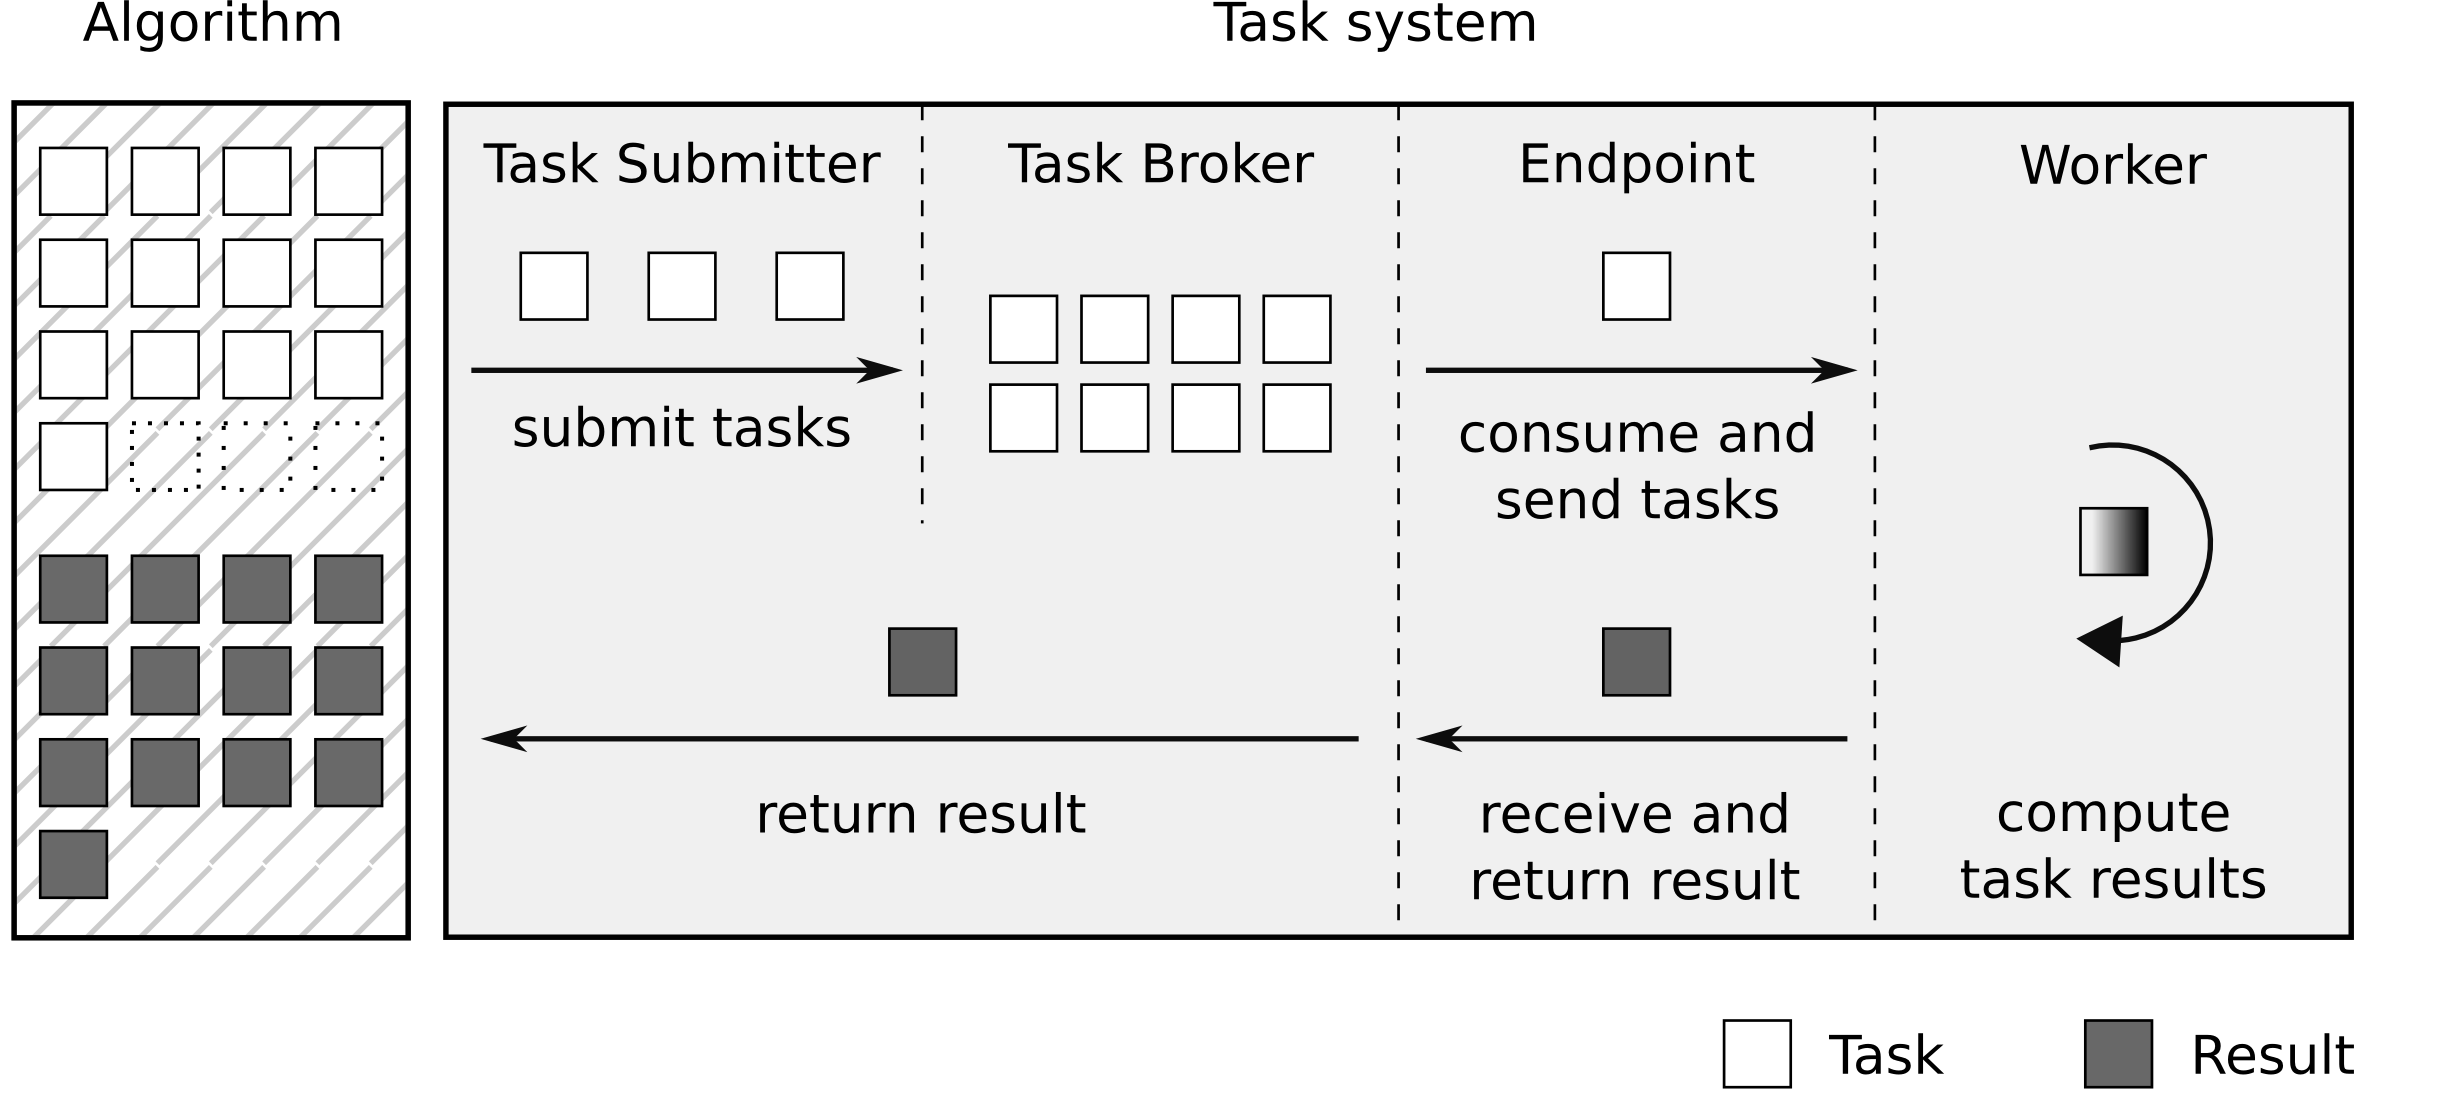
\includegraphics[width=130mm,natwidth=2438,natheight=1101]{task-system.png}
  \caption[Task submission to the task system]{Task submission to the task system. The task system consists of a task broker and any number of endpoints and workers. For the sake of simplicity, the figure shows only one endpoint and one worker. Here, an optional task submitter is used for task submission.}
  \label{fig:task-system}
\end{figure}

\subsection{Task Broker}
The task broker is the central feature in the task system. It is used to exchange tasks and their results between the algorithms and the endpoints. The broker combines an internal FIFO queue with additional task bookkeeping (see the concepts below).

All submitted tasks reference a task configuration that is used by the workers to compute the task result. This configuration can be shared by any number of tasks. The configuration reference for a given task is stored in the task broker. The configuration itself is sent to the workers on demand. A worker requests a specific task configuration, if it encounters a task whose configuration is unknown to the worker. After the configuration was received, it is cached by the worker for later reuse. The cache is only limited by the amount of available memory. This is appropriate, since usually many tasks use the same configuration. In the GA example, where the workers generate offsprings and compute their fitness values, a single task configuration is enough for all tasks, as offspring generation and fitness evaluation is done in the same way for all tasks. Therefore, a worker needs to obtain the task configuration only once, reducing the communication overhead. It is of course also possible to assign each task an individual task configuration. In this case, however, the communication overhead would increase, since task configurations have to be transmitted individually.

To work properly, the task broker uses two concepts that are needed to perform its work. The first concept is an internal first-in first-out (FIFO) queue, that stores the submitted tasks. The FIFO queue is thread safe, to allow multiple producers (algorithms) and consumers (endpoints) to interact with the queue at the same time. As an example, lets suppose that two GAs are running in one Biohadoop instance. Both algorithms can submit new tasks, while the endpoints consume tasks from the broker. By using a thread safe FIFO queue, all of this can happen simultaneously, without interfering with each other.

The second concept is a map connecting submitted tasks to their configuration and their \texttt{TaskFuture}. This is necessary, because a task loses its references once it is taken out of the FIFO queue and sent to a worker. The configuration for the task would become unknown and the result of the task could no longer be associated with the corresponding \texttt{TaskFuture}. The usage of a map resolves this problem.

The two concepts are depicted in figure \ref{fig:task-broker}. In the first step, a task $T_N$ and its configuration $TC_N$ is submitted to the broker. The broker inserts the task in its internal FIFO queue and adds the task, the configuration and a new \texttt{TaskFuture} $TF_N$ to its internal map. The \texttt{TaskFuture} is immediately returned to the algorithm as result of the task submission. At this stage, any attempt to access the result of the \texttt{TaskFuture} would block, as the result of the task computation is unknown yet. At a certain point, step 2 is performed, where the queued task $T_N$ is consumed by an endpoint and sent to a waiting worker. If the worker doesn't know about the referenced configuration $TC_N$ for task $T_N$, it asks the endpoint for the configuration, which gets the configuration from the broker in step 3. The configuration for the task $T_N$ can only be retrieved, because the broker kept a reference to it in its internal map. In step 4, the worker returns the computed result $R_N$ to the endpoint, which forwards it to the broker. The broker associates the result for task $T_N$ with the according \texttt{TaskFuture} $TF_N$ using its internal map. After the result for the \texttt{TaskFuture} is set, the algorithm can access the result $R_N$ for task $T_N$ without blocking.

\begin{figure}
  \centering
  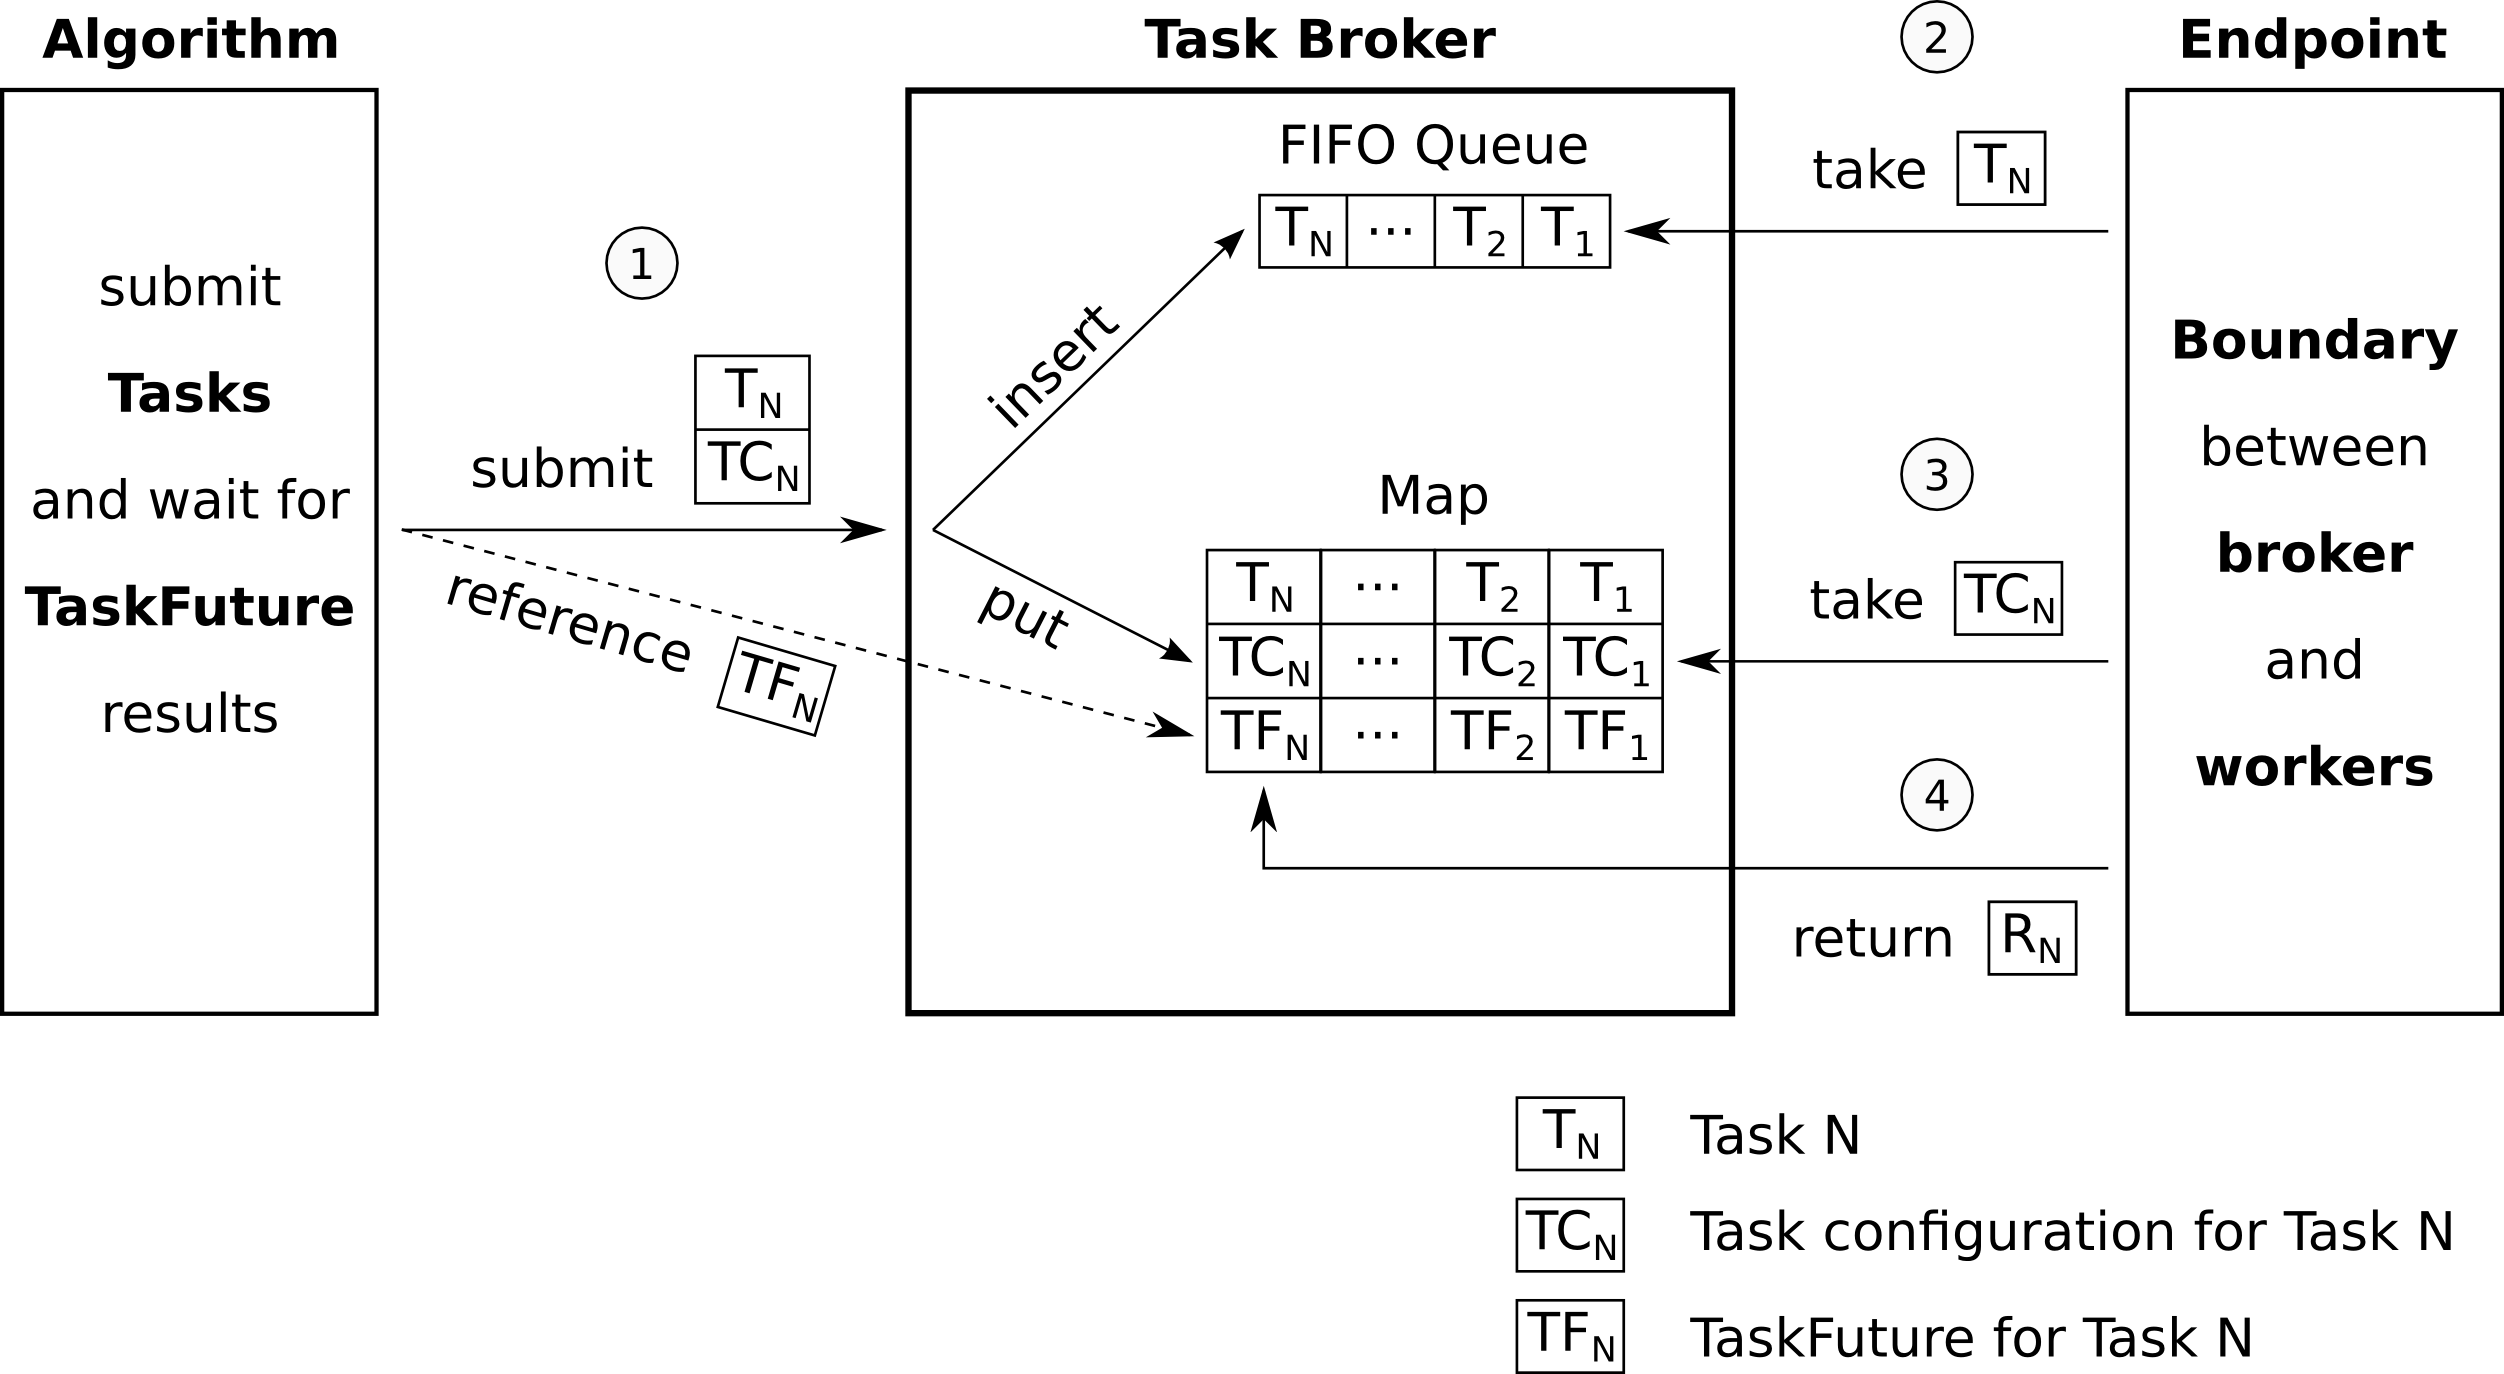
\includegraphics[width=130mm,natwidth=2504,natheight=1374]{task-broker.png}
  \caption[Internal structure of the task broker]{Internal structure of the task broker}
  \label{fig:task-broker}
\end{figure}

In addition to task and result exchange, the task broker provides methods to resubmit a task. This is needed in the case of a failure during the computation of the task result.

\subsection{Endpoint}
\label{chap:impl:endpoint}
An endpoint is a boundary between the task broker and the workers. It's main purpose is the communication with the workers. By hiding the technical details of the communication from the algorithm and the task broker, any type of communication facility between the master and the workers can be implemented. This property lead to the implementation of two different communication protocols for Biohadoop. Details about the communication can be found in section \ref{chap:impl:communication}.

Communication is not the only purpose of an endpoint. It interacts also with the task broker by taking tasks and task configurations out of it or returning results that were received from the workers. The attempt of an endpoint to get a task from the broker blocks, if the brokers internal FIFO queue is empty. As soon as new tasks are available, the endpoint continues to work. A blocked endpoint blocks also its waiting workers.

An endpoint is allowed to resubmit a task to the task broker if required. For example, lets suppose a task is taken from the task broker and sent to a worker. This worker encounters a problem and terminates before returning the result. The endpoint can detect the issue with different methods (e.g. connection closed, heartbeat, time out, etc.) and resubmits the task to the task broker. This way, no task gets lost.

It is possible to run an arbitrary amount of endpoints, but usually this is not necessary. Nevertheless, it can be useful to run different endpoints for different communication protocols (see section \ref{chap:impl:communication}).

The endpoints run in the YARN ApplicationMaster and are started and stopped automatically by Biohadoop. It is configurable which endpoints should be started, section \ref{chap:impl:configuration} gives details about the configuration aspects.

\subsection{Worker}
\label{chap:impl:worker}
A worker computes the result for a given task using the configuration that is referenced by the task. The task itself contains the data needed for the computation. The configuration contains information about how to compute the result for the task. The ``how'' is specified by a Java class that implements the \texttt{AsyncComputable} interface. In addition, the task configuration can contain an immutable data set, shared by all tasks that reference the same configuration. The immutable data set is called  ``initial data''.

In the GA example, a task generates and evaluates an offspring. The task data consists of the parent individuals and the task configuration points to a class that implements offspring generation and fitness evaluation. The ``initial data'' contains static parameters for offspring creation and fitness evaluation. The worker uses the configuration to instantiate the given \texttt{AsyncComputable} class. The class and the ``initial data'' are then used to compute the result for the task, which is a new offspring and its related fitness value. The result is then sent to the endpoint.

Tasks are sent to the workers without task configuration. The task configuration is delivered only on demand and is afterwards cached by the worker. This can be done, as most tasks will share a common configuration. Sending the configuration only on demand, reduces the amount of transmitted data and increases therefore the performance of the whole system. Figure \ref{fig:async-computable} shows how tasks and task configurations are handled by the workers.

\begin{figure}
  \centering
  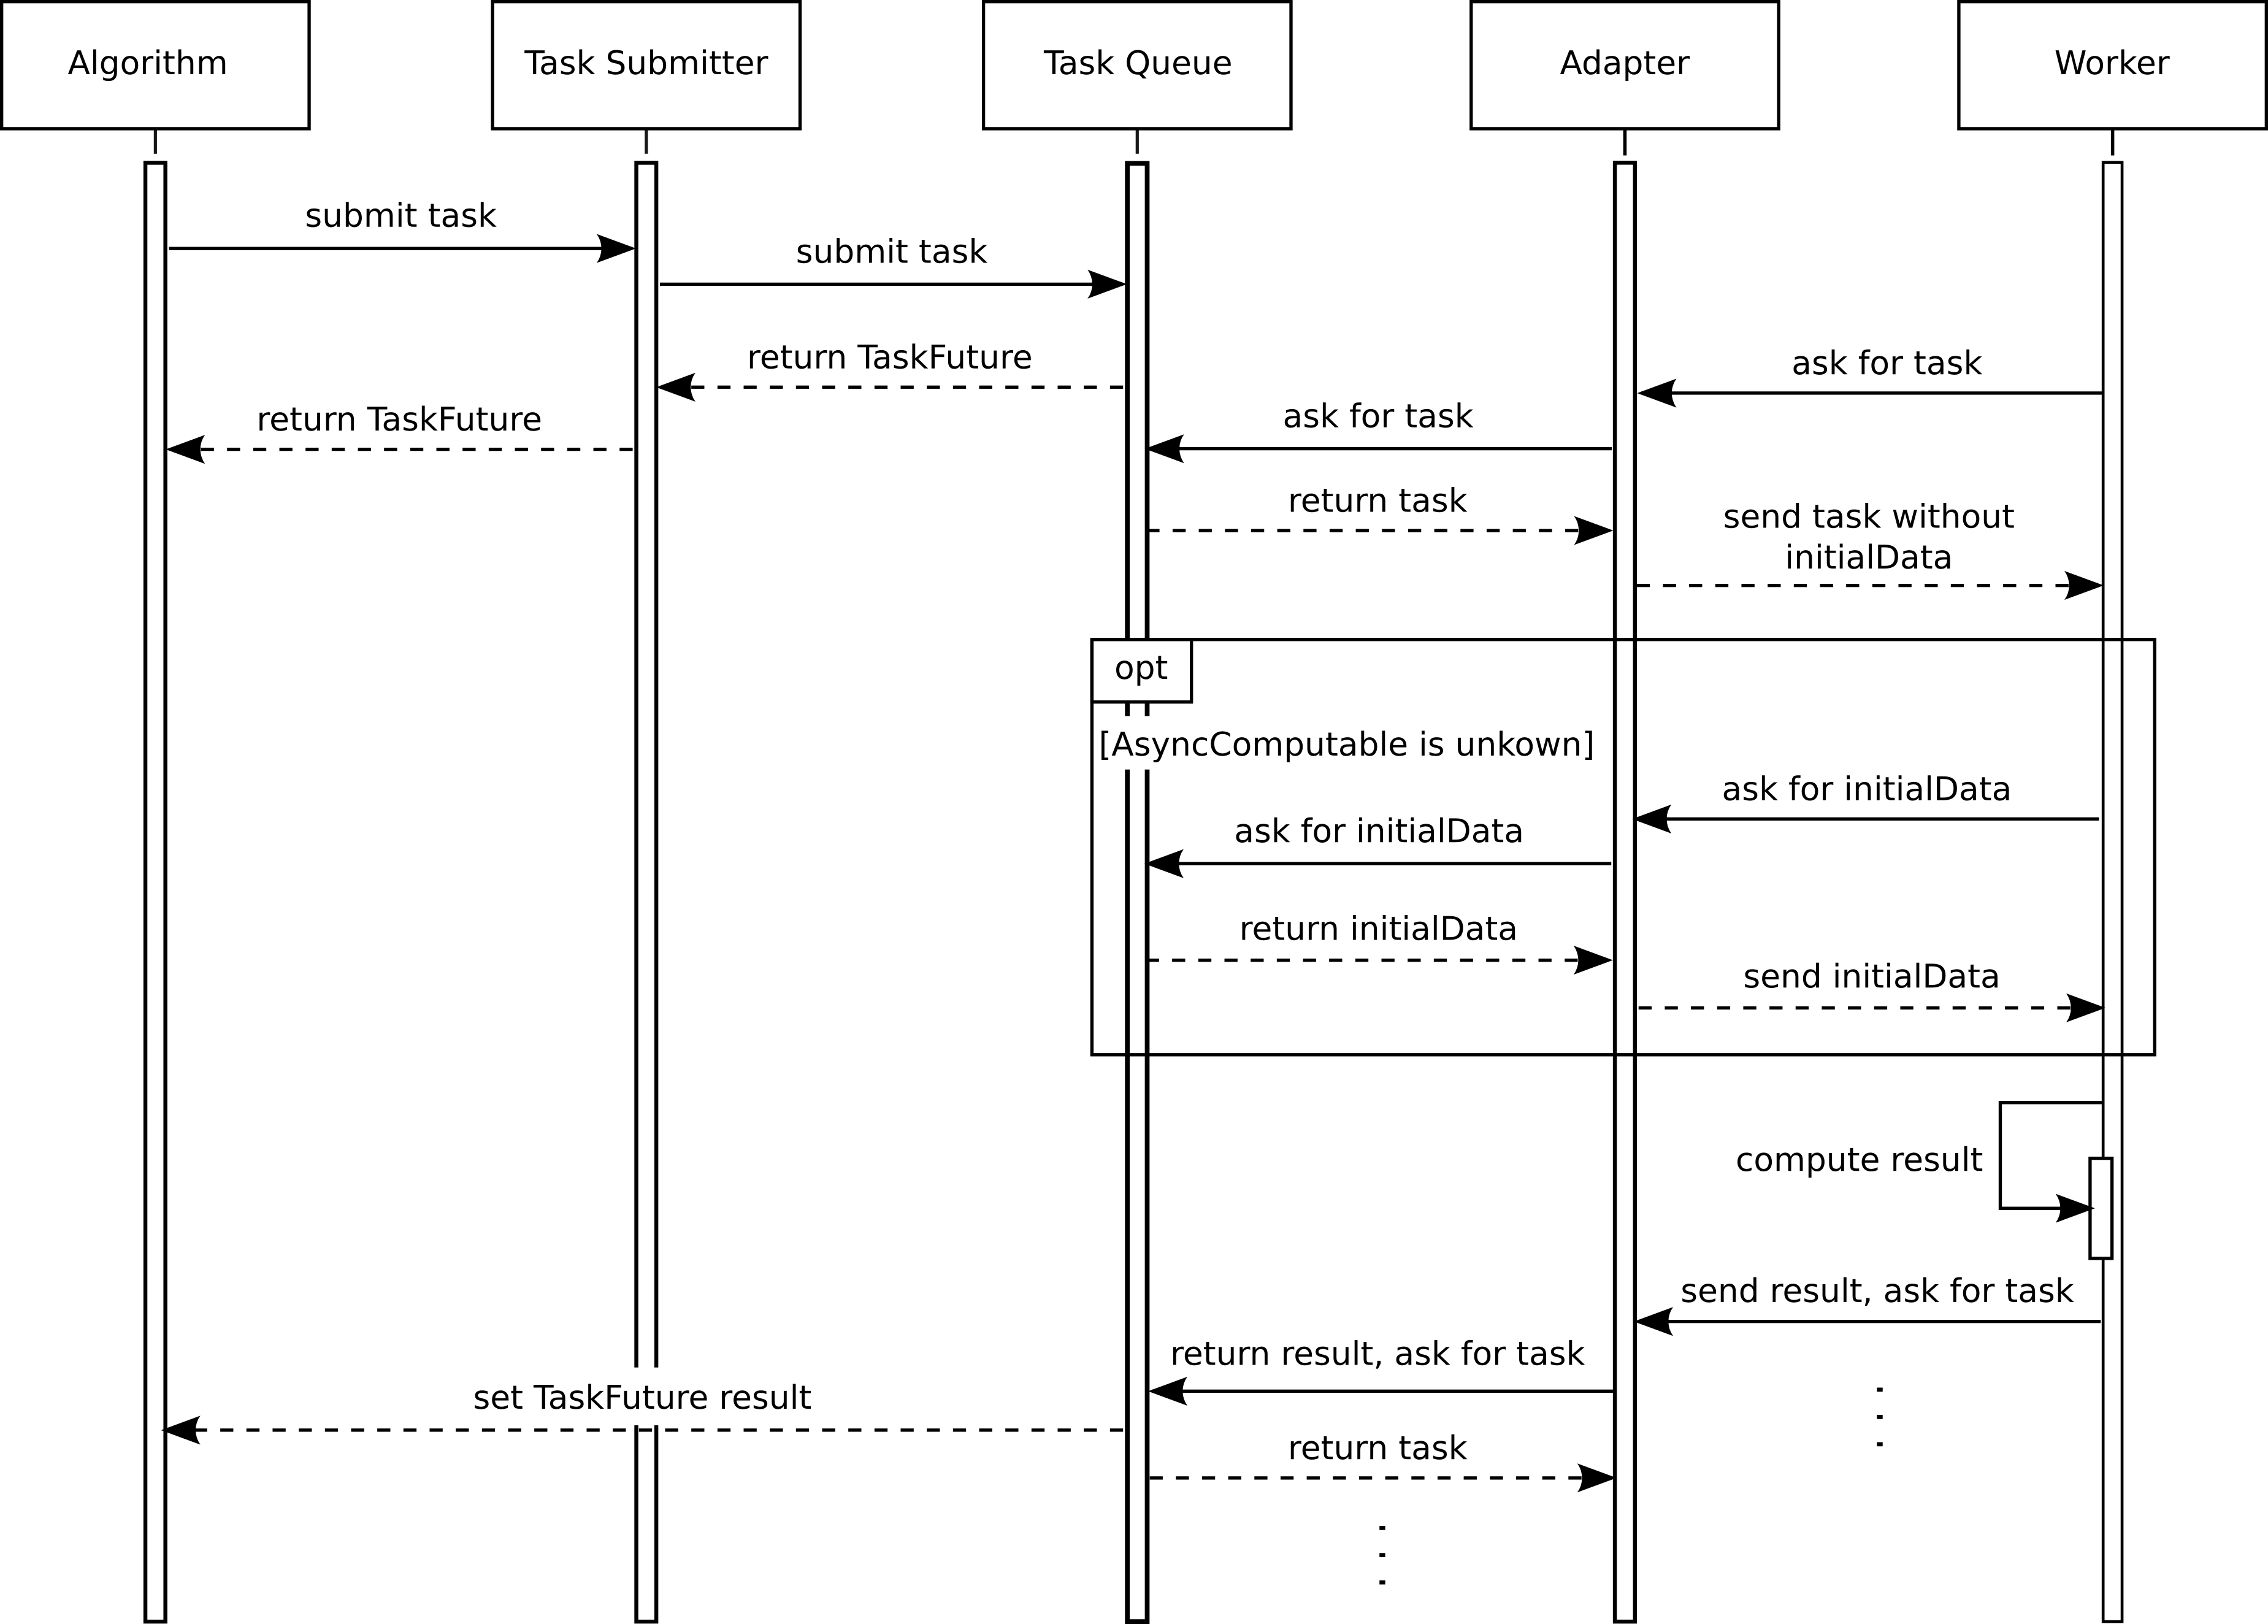
\includegraphics[width=130mm,natwidth=2901,natheight=2648]{flow-asyncComputable.png}
  \caption[Life cycle of a task]{Life cycle of a task. The result is computed by a worker using an \texttt{AsyncComputable}.}
  \label{fig:async-computable}
\end{figure}

A worker needs to communicate with an endpoint to get tasks. If the endpoint has currently no work to offer, for example because the running algorithms have not submitted any tasks to the task system, then the worker waits until new work is available. Of course the worker need some resources during the waiting times too, like CPU, RAM and storage or, in YARN terms, containers. One should consider and measure how many workers are really needed.

Biohadoop supports two different kinds of workers: the ones that run under the control of the Apache Hadoop system (from now on called ``embedded workers'') and the ones that run outside of this system (from now on called ``external workers'').

Embedded workers must be configured in Biohadoop, which controls their life cycle. In contrast, external workers can not be configured by Biohadoop, their whole life cycle must be controlled in some other way that is not part of Biohadoop. This can pose some problems, as external workers need to know, e.g., when and where Biohadoop is running. The solution to this problems is outside of the scope of this thesis.

For most applications embedded workers are just fine. There are, however, some good reasons to use external workers:

\begin{itemize}
  \item External worker don't necessarily depend on the Hadoop ecosystem, they may run wherever they want, as long as they are able to communicate to at least one endpoint. It is possible to develop external workers that run in completely different environments, for example on mobile phones.
  \item There is no restriction on the programming language for an external worker, as long as it knows how to talk to an endpoint. For example it is possible to implement a worker in JavaScript \footnote{\url{https://github.com/gappc/bioworker-browser} last access: 07.01.2015} or Python.\footnote{\url{https://github.com/gappc/bioworker-python} last access: 07.01.2015} In contrast, embedded workers have to be written in Java.
  \item There is no limit to the number of external workers that may run. On the other side, the number of embedded workers is limited by the Hadoop environment on which Biohadoop runs.
\end{itemize}

Biohadoop provides the possibility to run different endpoints to support external workers. The endpoints may implement arbitrary communication protocols, e.g., WebSockets with JSON serialization for external workers written in JavaScript.

\section{Communication}
\label{chap:impl:communication}
The communication between the algorithms, the broker and the endpoints is not difficult, as they run in the YARN ApplicationMaster and therefore in the same JVM. It is just a matter of sharing variables between the different threads, possibly protected by concurrency protocols. For example, the task broker contains a FIFO queue based on the Java \texttt{LinkedBlockingQueue}, which is a thread safe queue that supports concurrent writers and readers.
  
Communicating between endpoints and workers is more complicated, as the endpoints and workers may run in different processes or even on different machines, which makes variable sharing more difficult. A more sophisticated communication method must be used.

Biohadoop uses Netty \footnote{\url{http://netty.io/} last access: 19.11.2014} for all communication purposes that span different processes or machines. Netty is a high performance framework for network applications that hides the underlying socket implementation from the user and provides a useful and well tested API to build distributed applications. Although, Netty provides TCP and UDP support, only TCP is used for Biohadoop. All provided endpoints and workers use Netty as their communication base.

The communication protocols on top of Netty can be of arbitrary type. Biohadoop provides two implementations for endpoints and workers that use sockets (hidden by Netty) or the WebSocket protocol. The socket protocol uses Kryo \footnote{\url{https://github.com/EsotericSoftware/kryo} last access: 04.08.2014} for object serialization, while the WebSocket protocol relies on JSON serialization. The two protocols are discussed in more detail in section \ref{chap:impl:protocols}.

The reason for the support of different protocols lies in their different use cases. While the performance of sockets with Kryo serialization is higher than for WebSockets, WebSockets have the advantage of great compatibility and broad support in different languages. This is important for external workers as they don't have to be implemented in Java.

On top of the communication protocols, Biohadoop establishes its own application protocol for task, configuration and result exchange between endpoints and workers. This protocol defines a communication flow further described in section \ref{chap:impl:communication-flow}. Figure \ref{fig:communication-layers} shows the different layers used by Biohadoop for data exchange.

\begin{figure}
  \centering
  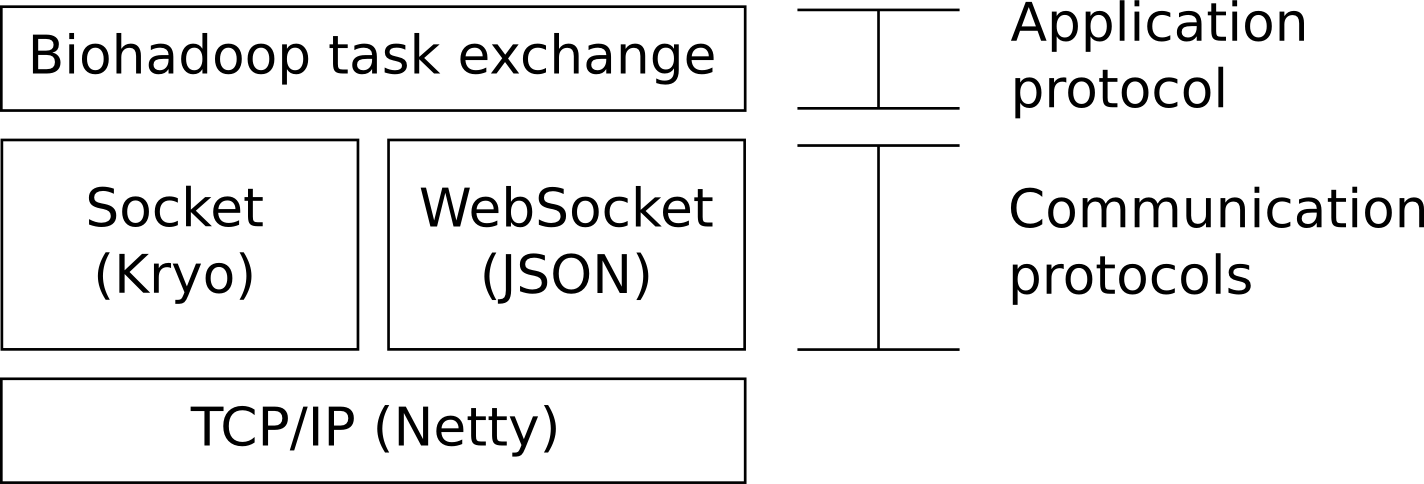
\includegraphics[width=80mm,natwidth=1424,natheight=484]{communication-layers.png}
  \caption[Biohadoops communication layers]{Biohadoops communication layers}
  \label{fig:communication-layers}
\end{figure}

Biohadoop enables the use of custom protocols, by implementing the appropriate parts of \texttt{Endpoint} and \texttt{Worker} interfaces. Corresponding endpoints and workers have to agree about the communication and application protocol.

\subsection{Protocols}
\label{chap:impl:protocols}
In this section, the two provided communication protocols of Biohadoop are described, each one has its advantages and disadvantages.

\subsubsection{Sockets}
The socket communication between endpoints and workers is implemented on top of Netty that provides an abstraction of the underlying raw TCP/IP socket. The advantage of using Netty over raw sockets is, that Netty provides a simple to use API for non-blocking asynchronous communication. A manual implementation is typically more error prone.

Kryo is used for object serialization. It is a library for high speed serialization of Java objects and is usually faster than the build-in serialization features of Java.\footnote{\url{https://github.com/eishay/jvm-serializers/wiki} last access: 27.11.2014}

A disadvantage of Kryo is, that its object serialization is not a standard and therefore in broad usage. This restricts the worker implementations to be written in Java, which may not be a problem at all, especially if only embedded workers are used. However, if external workers should be used, they have to be written in Java, or need to provide a custom Kryo implementation.

If the data exchanged between endpoints and workers is huge, the Kryo buffer sizes must be increased. This can be done by setting the according configuration options in the configuration file (see section \ref{chap:impl:configuration}).

\subsubsection{WebSocket}
The WebSocket implementation also uses Netty to hide the underlying TCP/IP socket. In contrast to the socket communication, it adds the WebSocket protocol on top of it. JSON is used for object serialization.

WebSockets are usually used for the communication between a web application and its application server. They rely on the HTTP protocol for the handshake, during which the communication partners agree to upgrade to the WebSocket protocol. After the upgrade is done, the communication between an endpoint and a worker can be performed using binary streams or text streams.

WebSockets have a very small overhead when data is exchanged, e.g., 2 Bytes for text stream messages. This is a major difference to the HTTP protocol where the larger HTTP headers are sent on each request and response. It improves the communication performance, especially for the transmission of small amounts of data. Another difference between WebSockets and HTTP is, that the WebSocket communication can be performed in full duplex, HTTP needs a request - response cycle. This can further improve the performance, but has no impact for Biohadoop, as the communication between endpoints and workers is performed in a request - response manner (see section \ref{chap:impl:communication-flow} for more information).

The biggest advantage of WebSockets and JSON lies in their standardization. This is important in combination with external workers, as those workers can be written in any language. Most languages have support for WebSockets and JSON, since they are standardized. The biggest disadvantage of WebSockets with JSON is, that they are slower than sockets with Kryo serialization.

\subsection{Communication Flow}
\label{chap:impl:communication-flow}
The communication protocols presented in the prior section are used as a base to the application protocol, that implements a well defined communication flow between endpoints and workers. This communication flow, depicted in figure \ref{fig:communication-flow}, is the same for both communication protocols available. Custom protocols don't need to implement this flow, they are free to implement their own communication pattern.

\begin{figure}
  \centering
  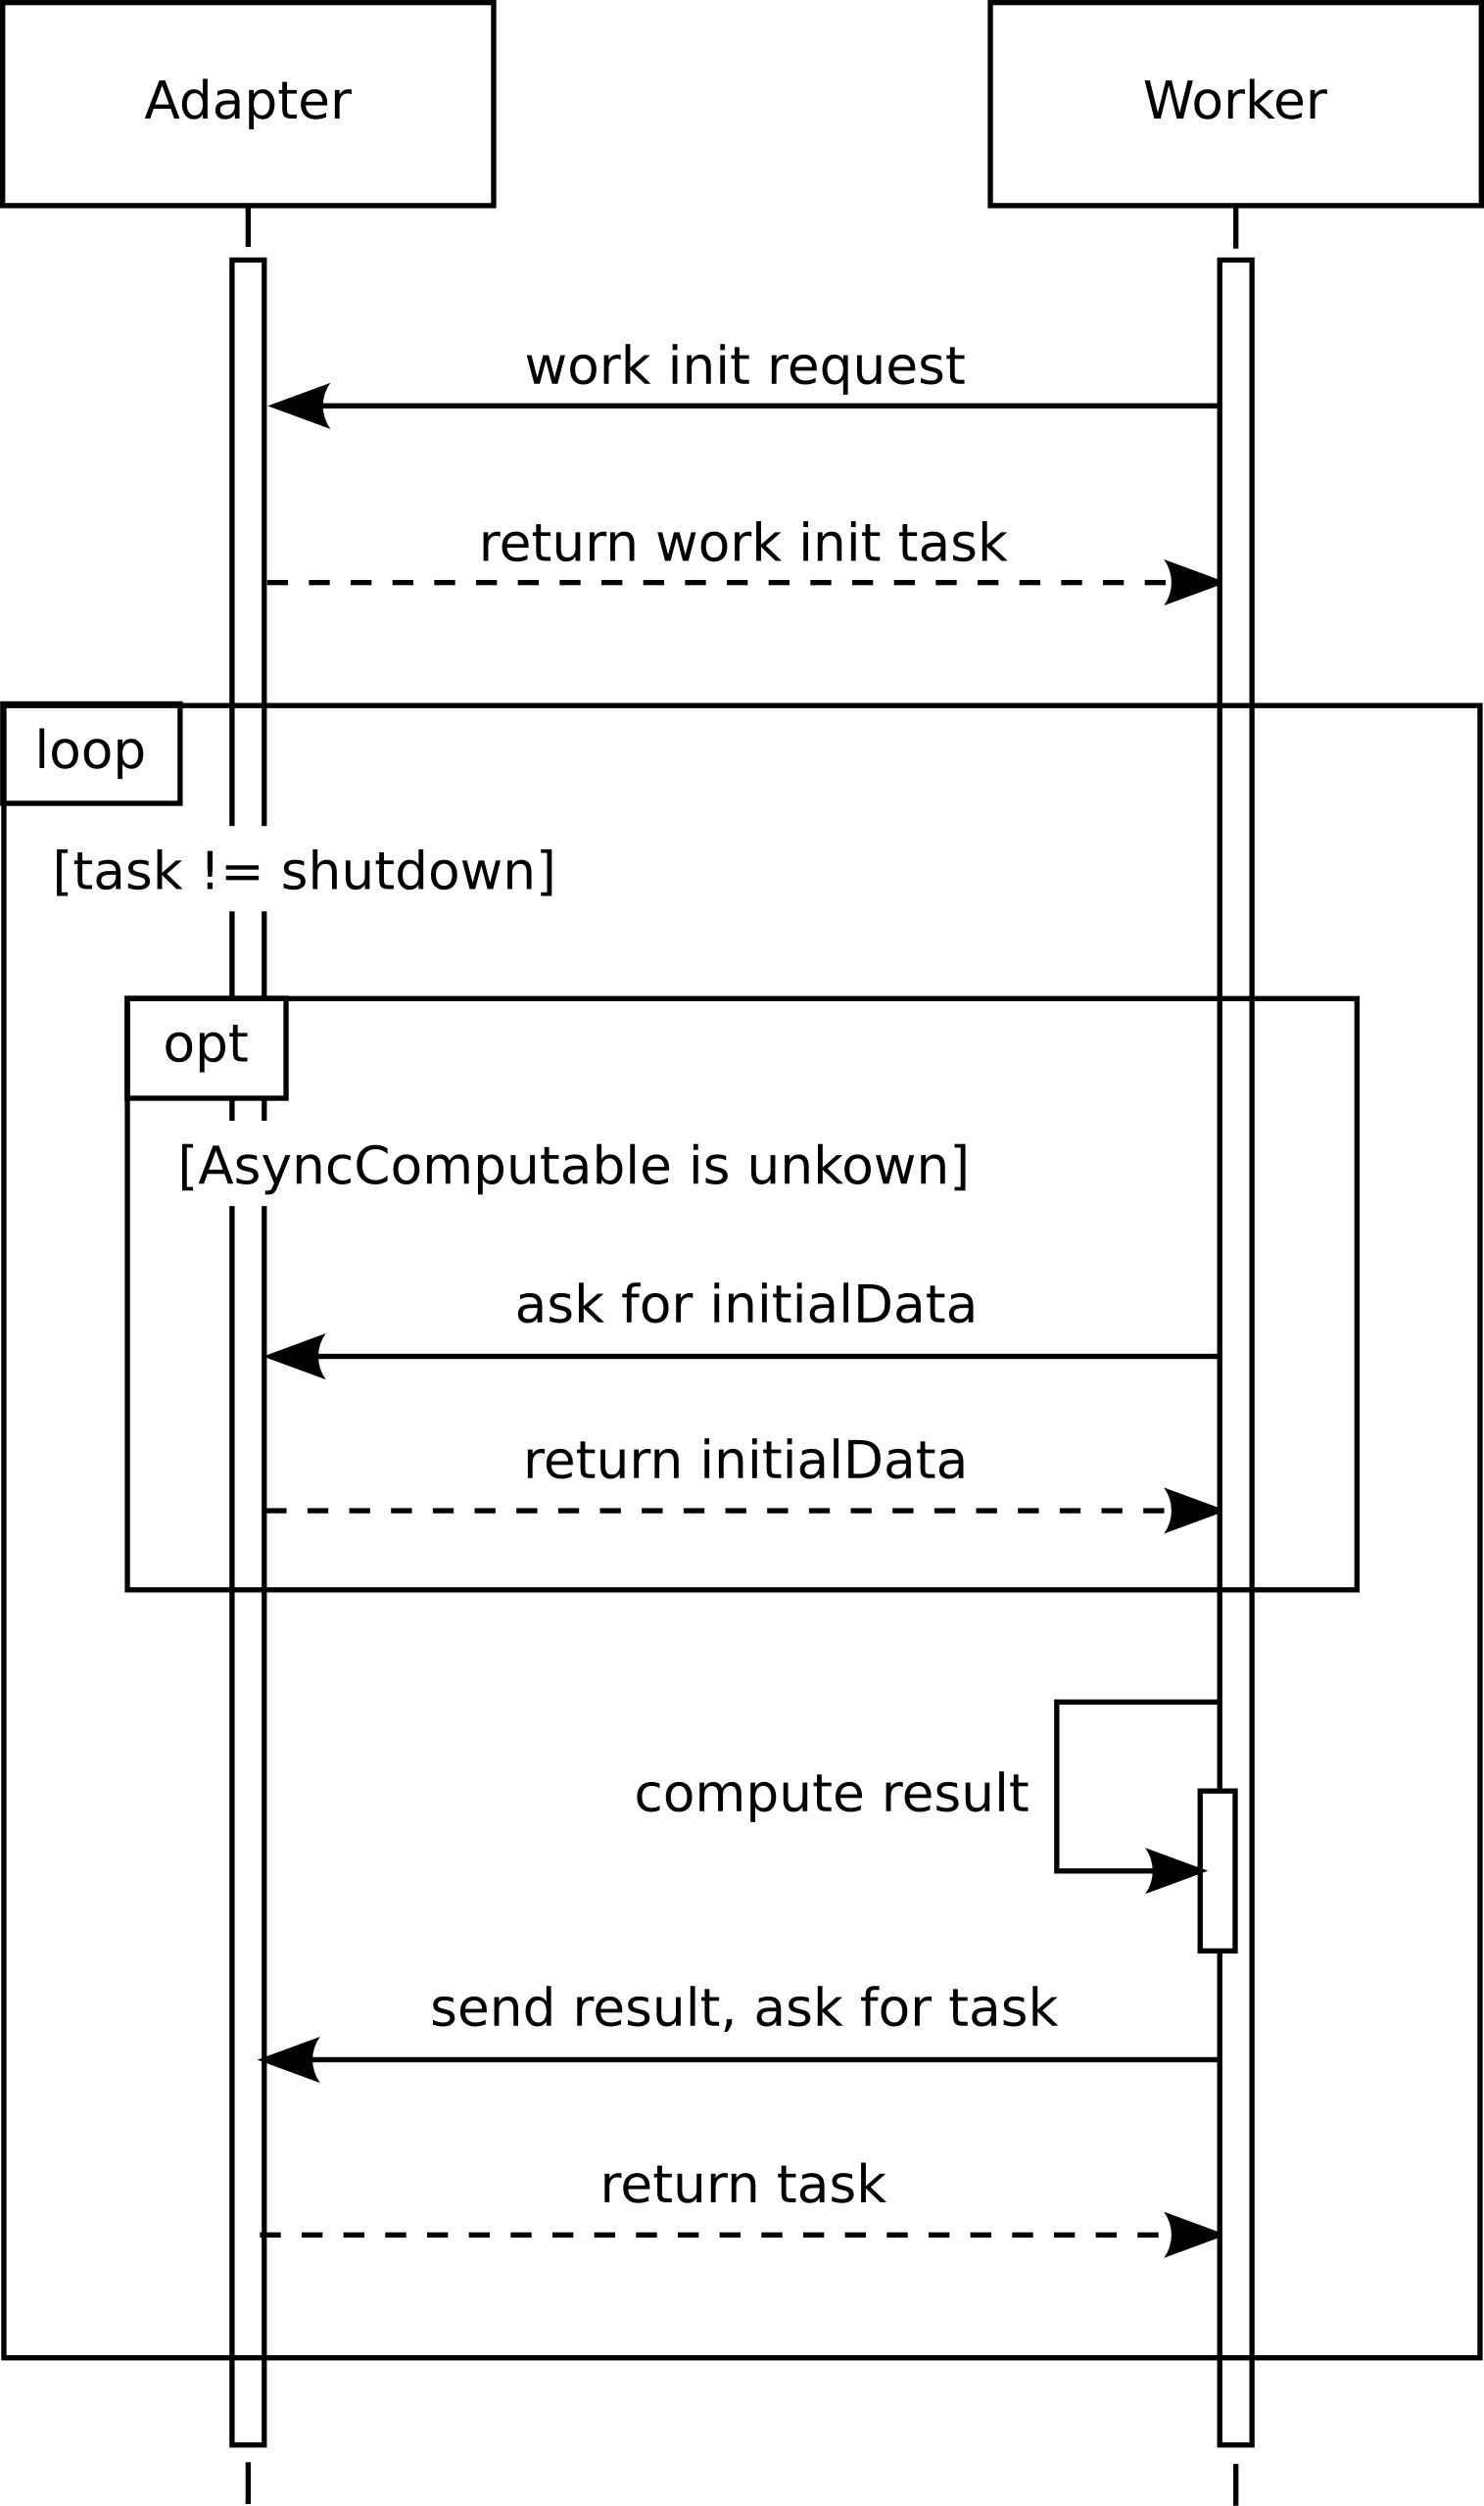
\includegraphics[width=70mm,natwidth=1515,natheight=2216]{communication-flow.png}
  \caption[Communication flow between endpoints and workers]{Communication flow between endpoints and workers}
  \label{fig:communication-flow}
\end{figure}

As one can see in figure \ref{fig:communication-flow}, the communication between endpoints and workers is initialized by the worker. After the worker gets a task from an endpoint, it looks if the needed task configuration is already stored in its internal cache. If the configuration is unknown, the worker requests it from the endpoint. The endpoint responds with the configuration, which is cached by the worker for further reuse. The worker computes the result for the task using the task data, and the corresponding configuration. The result is then transmitted to the endpoint and a new task is requested.

\section{Extensions}
\label{chap:impl:extensions}
Biohadoop provides two extensions for algorithms, beside the task system presented in section \ref{chap:impl:task-system}. The first one is for persistence, where it is possible to load and store arbitrary data to and from a file system (see section \ref{chap:impl:persistence}). The second extension provides high level parallelism between parallel running algorithms, called the ``island model'' (see section \ref{chap:impl:island-model}).

\subsection{Persistence}
\label{chap:impl:persistence}
There are a lot of reasons to store algorithm results to a file system. The most important is to save the final result of a computation. Another reason is to store intermediate results in case something happens. If this data is reloaded afterwards, the computation can continue from that point on. Intermediate results can also be used for other computations or for visualization.

The conclusion is that some kind of persistence is useful. It should include both the saving and loading of data. Biohadoop provides this kind of service by offering a simple API accessible through the class \texttt{FileUtils}. The API stores provided data in JSON format in a file with a given name. When a file is loaded, the API supposes that the contained data is also in JSON format and tries to deserialize it. An exception is thrown if this is not possible.

Although, the API covers the fundamental persistence use cases, a programmer is free to use its own mechanism of data storage and retrieval.

\subsection{The Island Model}
\label{chap:impl:island-model}
% The island model is a high level parallelization model that is sometimes used in optimization problems. In the island model, several algorithms run in parallel, trying to compute the result to the same problem. The parallel running algorithms are called the islands. Each of these algorithms is independent of the others, and each one may have a different solution at a given point of time. By exchanging their data after some intervals, islands may get interesting solutions from other islands that can be integrated in their own computation to enhance their solution. If we take the GA as an example, the islands would consist of independently running GAs that exchange individuals to improve the solution. Figure \ref{fig:island-model} shows an example island model with 3 GAs that exchange individuals.
% 
% \begin{figure}
%   \centering
%   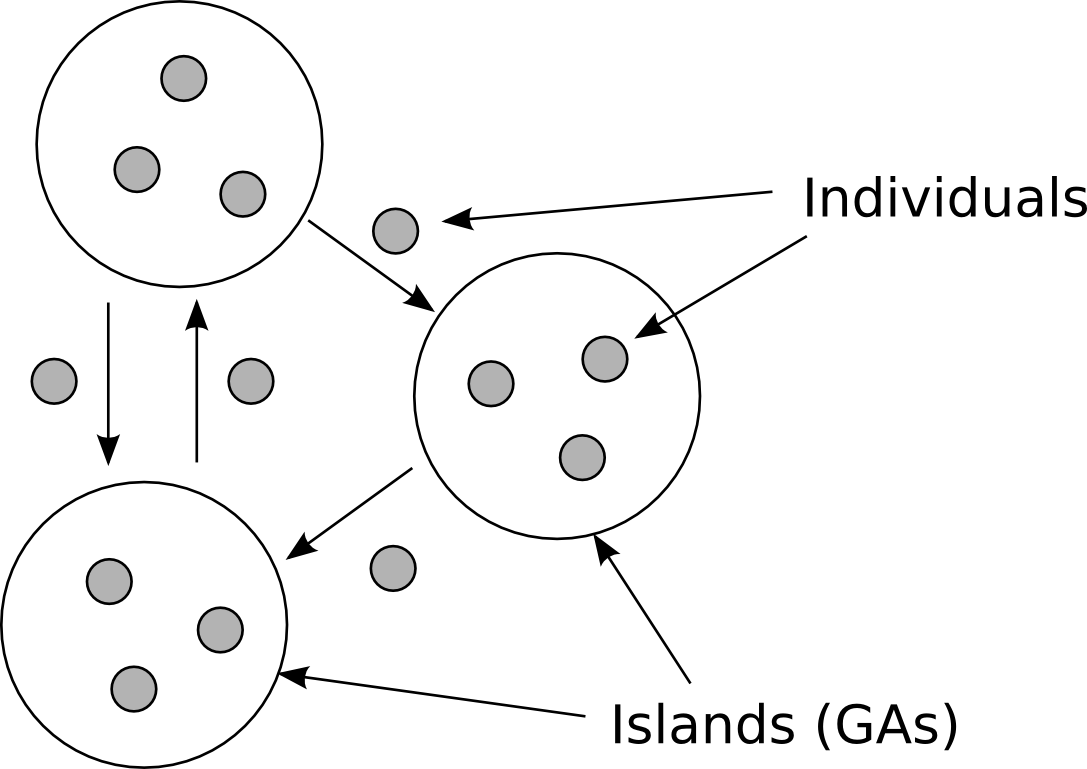
\includegraphics[width=70mm]{island-model.png}
%   \caption{Example island model with 3 GAs, exchanging individuals}
%   \label{fig:island-model}
% \end{figure}
% 
% The island model enhances the exploratory behavior of optimization algorithms, which often results in better overall solutions. As the data exchange is only done at certain points of time, the islands have the chance to exploit their own solution. When they get stuck in a local optima, they get the chance to escape this optima by considering solutions from other islands.
% 
Biohadoop provides an API, implemented in the class \texttt{IslandModel}, that can be used to build an island model between any number of algorithms. It provides methods to register to ZooKeeper, publish the own solutions to other islands or to merge remote solutions with the own solutions. Data merging can be configured by implementing the interfaces \texttt{RemoteResultGetter} and \texttt{DataMerger}. The \texttt{RemoteResultGetter} defines from which remote island the data should be retrieved. It may take into account different properties, like the number of iterations, the fitness of individuals, etc. The \texttt{DataMerger} defines, how two solutions should be merged.

The island model API uses ZooKeeper, which is a server that provides distributed configuration and synchronization services and a naming registry. Therefore, a running ZooKeeper instance must be accessible by Biohadoop, if an algorithm wants to use the island model.

By using ZooKeeper as central registry for the island model, it doesn't matter if the algorithms run in the same Biohadoop instance or in different Biohadoop instances. They find each other through their ZooKeeper registrations.

The main advantage of running several algorithms in the same Biohadoop instance is, that it guarantees that they all run simultaneously. Scheduling several Biohadoop instances in parallel doesn't guarantee that they also run in parallel, as YARN decides when an application is launched. The island model is useless if the algorithms don't run at the same time.

\section{Configuration}
\label{chap:impl:configuration}
Biohadoop uses a configuration file in JSON format. The advantage of JSON is, that its understandable for humans and usually smaller in size than, e.g., XML.

The path to the configuration file must be given on invocation of Biohadoop as its first parameter (more information on how to run Biohadoop can be found in appendix \ref{chap:usage:run}). Biohadoop stops immediately with an exception if the path is empty, not existing or the configuration file can not be parsed.

The configuration file itself consists of the following four top-level objects:
\begin{description}
  \item[communicationConfiguration]: Defines a list of endpoints and a list of workers that Biohadoop should start. The worker configuration provides additional information about the number of workers that should be started.
  \item[globalProperties]: A map of keys and values as strings. This properties are used for global settings that should be available in the ApplicationMaster. Examples for such global settings are configurations for Kryo and ZooKeeper.
  \item[includePaths]: A list of strings that defining the paths where needed libraries can be found. This isn't important for a locally running instance of Biohadoop (e.g. during development), as the necessary classpaths must be set when starting Biohadoop. It is, however, important when Biohadoop runs in the Hadoop environment, since these are the paths to libraries that Hadoop should provide to Biohadoop when running. If the paths to the necessary libraries are wrong when running on Hadoop, Biohadoop won't run correctly.
  \item[algorithmConfigurations]: a list of algorithms that should be run by Biohadoop. Each element in the list describes the configuration for an algorithm. The configured algorithms are started in parallel in the same Biohadoop instance.
\end{description}

Although possible, it is not always convenient to write a configuration by hand. Biohadoop provides two builder classes to simplify the generation of configuration files. The builder in \texttt{BiohadoopConfiguration} offers methods to configure the top level elements of a configuration file. Algorithm configuration is simplified by the builder in \texttt{AlgorithmConfiguration}. The result of this algorithm configuration can then be handed over to the \texttt{BiohadoopConfiguration} builder.

\section{Biooozie}
\label{chap:impl:oozie}
Biooozie implements a custom action for Apache Oozie (see section \ref{chap:hadoop:oozie}) that schedules one or several instances of Biohadoop. The action can be part of a workflow of arbitrary size. The outcome of the custom action is ``ok'' if no error happened during the execution of the action. This is also true for the case that several Biohadoop instances are defined in one action. If any Biohadoop instance fails, the outcome of the action is ``error''.

A short example workflow with three stages copies data sets to a HDFS file system, on which some MapReduce action is performed that produces new data sets. Those data sets in turn are the basis for a GA computation, performed by Biohadoop (see figure \ref{fig:biooozie}).

\begin{figure}
  \centering
  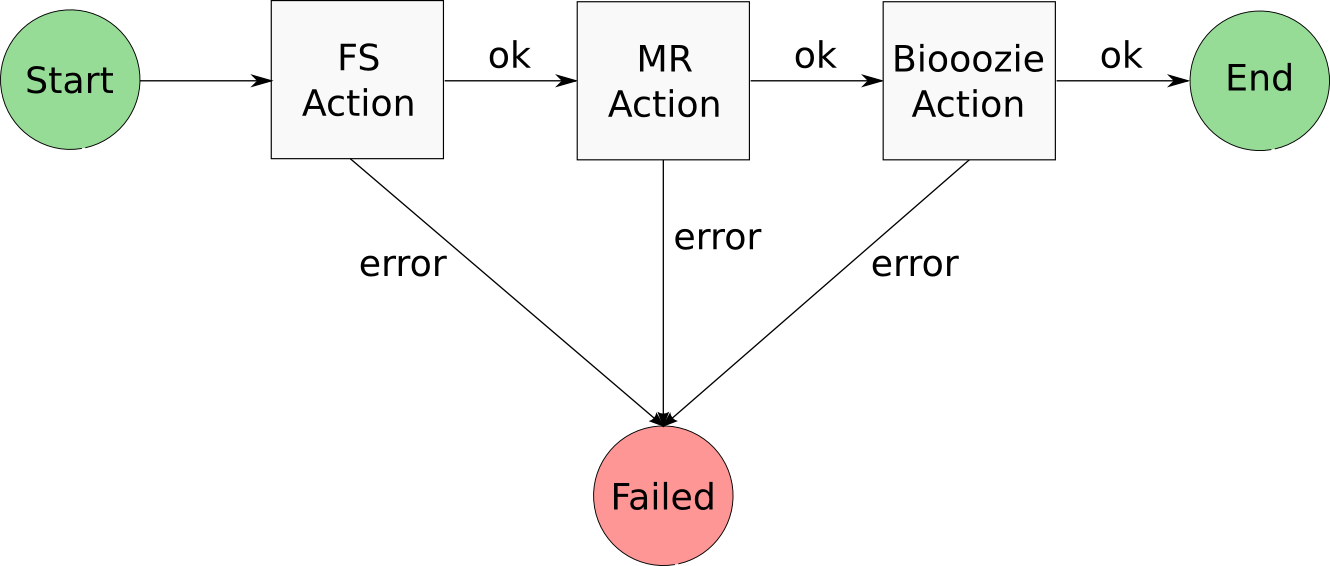
\includegraphics[width=100mm,natwidth=1330,natheight=566]{biooozie.png}
  \caption[Oozie workflow, including Biooozie action]{Example Oozie workflow, including Biooozie action}
  \label{fig:biooozie}
\end{figure}

The action is configured in an Oozie workflow as an XML element named \texttt{biohadoop}. It contains one \texttt{name-node} element that defines the URL of the HDFS NameNode, and one or several \texttt{config-file} elements. Each \texttt{config-file} element represents a Biohadoop instance that starts with the given configuration file. This way it is possible to schedule several Biohadoop instances in parallel, using a single action. The parallel instances are for example useful for running an island model.

The term ``schedule'' is used here on purpose, because Hadoop doesn't guarantee that the instances also run in parallel, this depends on the available Hadoop resources, i.e., on the available YARN containers. It is for example possible that a custom action schedules three instances of Biohadoop, but due to a lack of Hadoop resources, the instances run sequentially.

Biohadoop could also be invoked using Oozies \texttt{java} action, the advantage of Biooozie is that its tailored to Biohadoop and there is no need to provide all the parameters that a simple \texttt{java} action needs. 